\chapter{SYSTEM DESIGN}
\label{chap:system_design}
\renewcommand{\floatpagefraction}{0.6}

The UML diagrams below use the class, endpoint and table names of the \texttt{Backend\_API}, \texttt{Admin\_Web\_Panel} and \texttt{Student\_Desktop\_App} projects.

\section{Structure Diagrams}
Structure diagrams show the static parts of a system: its classes, components and machines \cite{structure_diagram_techopedia}. Agreeing on them early let us build the client, panel and API in parallel.

\subsection{Class Diagram}
\begin{sloppypar}
A class diagram shows classes, their attributes and their associations \cite{class_diagram_uml, class_diagram_sparx}. The design is drawn in three parts. Figure~\ref{fig:class_diagram} shows the core entities, which are Entity Framework Core classes in \texttt{Backend\_API/Models}. Each student has at most one \texttt{DeviceBinding}, which ties the account to one workstation. A teacher owns exams through the sections they teach, and \texttt{ExamProctor} links invigilators to exams; these two links are the owner and proctor rules of \texttt{ExamAccessService}.
\end{sloppypar}

\begin{figure}[!htbp]
\centering
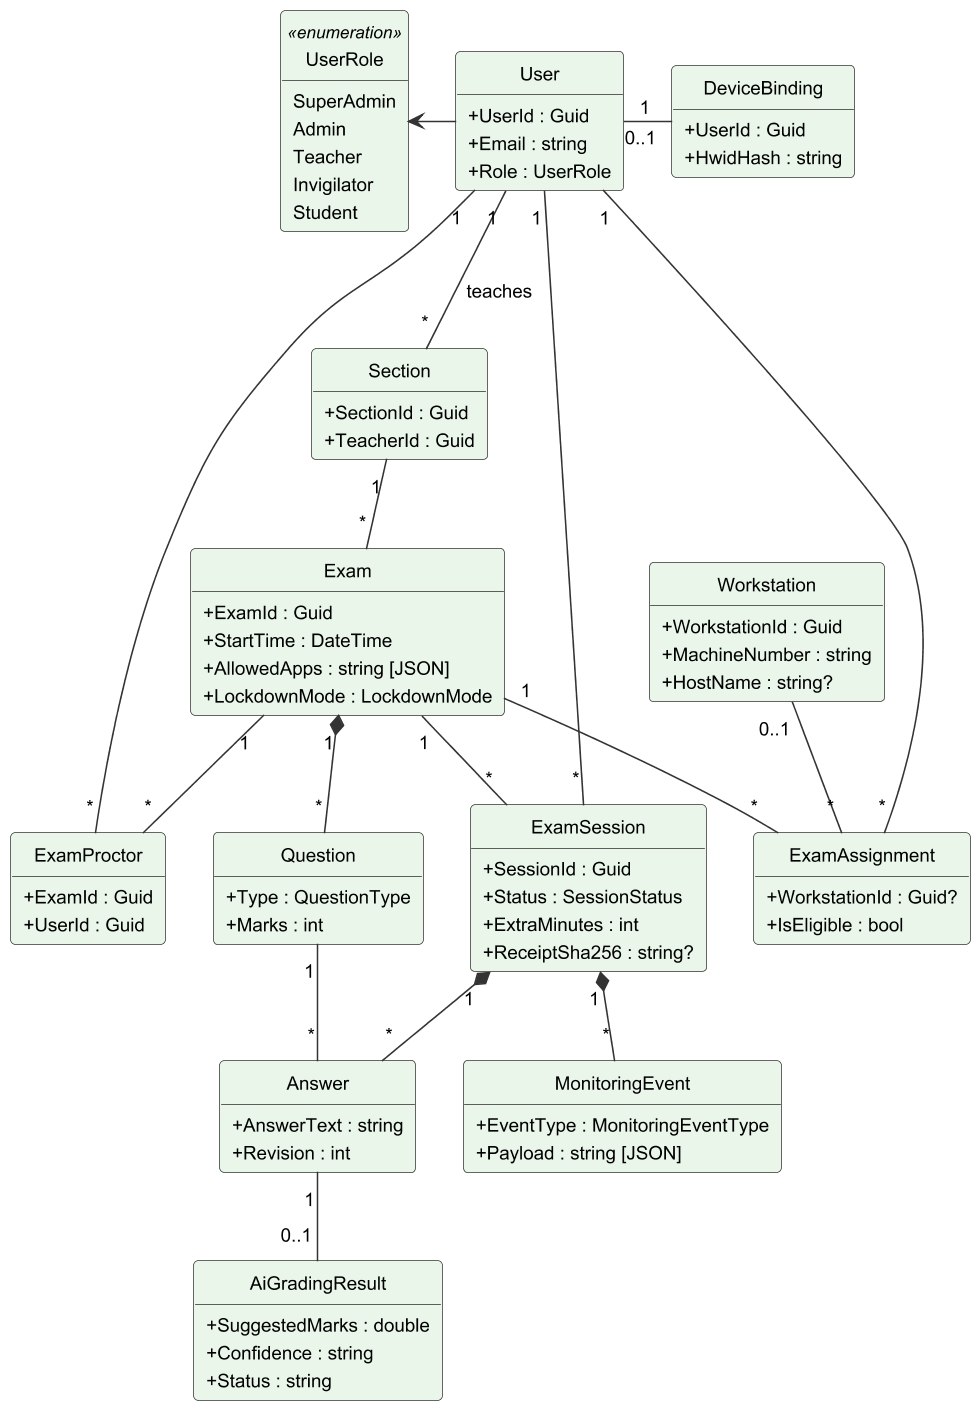
\includegraphics[width=0.72\linewidth]{Figures/class_diagram.png}
\caption{Class Diagram of the SmartExam Data Model}
\label{fig:class_diagram}
\end{figure}

\begin{sloppypar}
In the desktop app (Figure~\ref{fig:class_diagram_client}) \texttt{LockdownCoordinator} holds the keyboard, process, clipboard, device and Task Manager guards and reports violations to \texttt{LiveMonitoringService}, which owns the webcam monitor with the YuNet and YOLOX-Nano models. \texttt{ApiClient} is the only class that calls the server. On the server (Figure~\ref{fig:class_diagram_server}) the controllers use \texttt{ExamAccessService}, \texttt{SeatGuard} and \texttt{SubmissionService}; \texttt{GradingWorker} takes queued answers and calls \texttt{GradingService}, which picks a Docker or MinGW \texttt{ICodeRunner}.
\end{sloppypar}

\begin{figure}[!htbp]
\centering
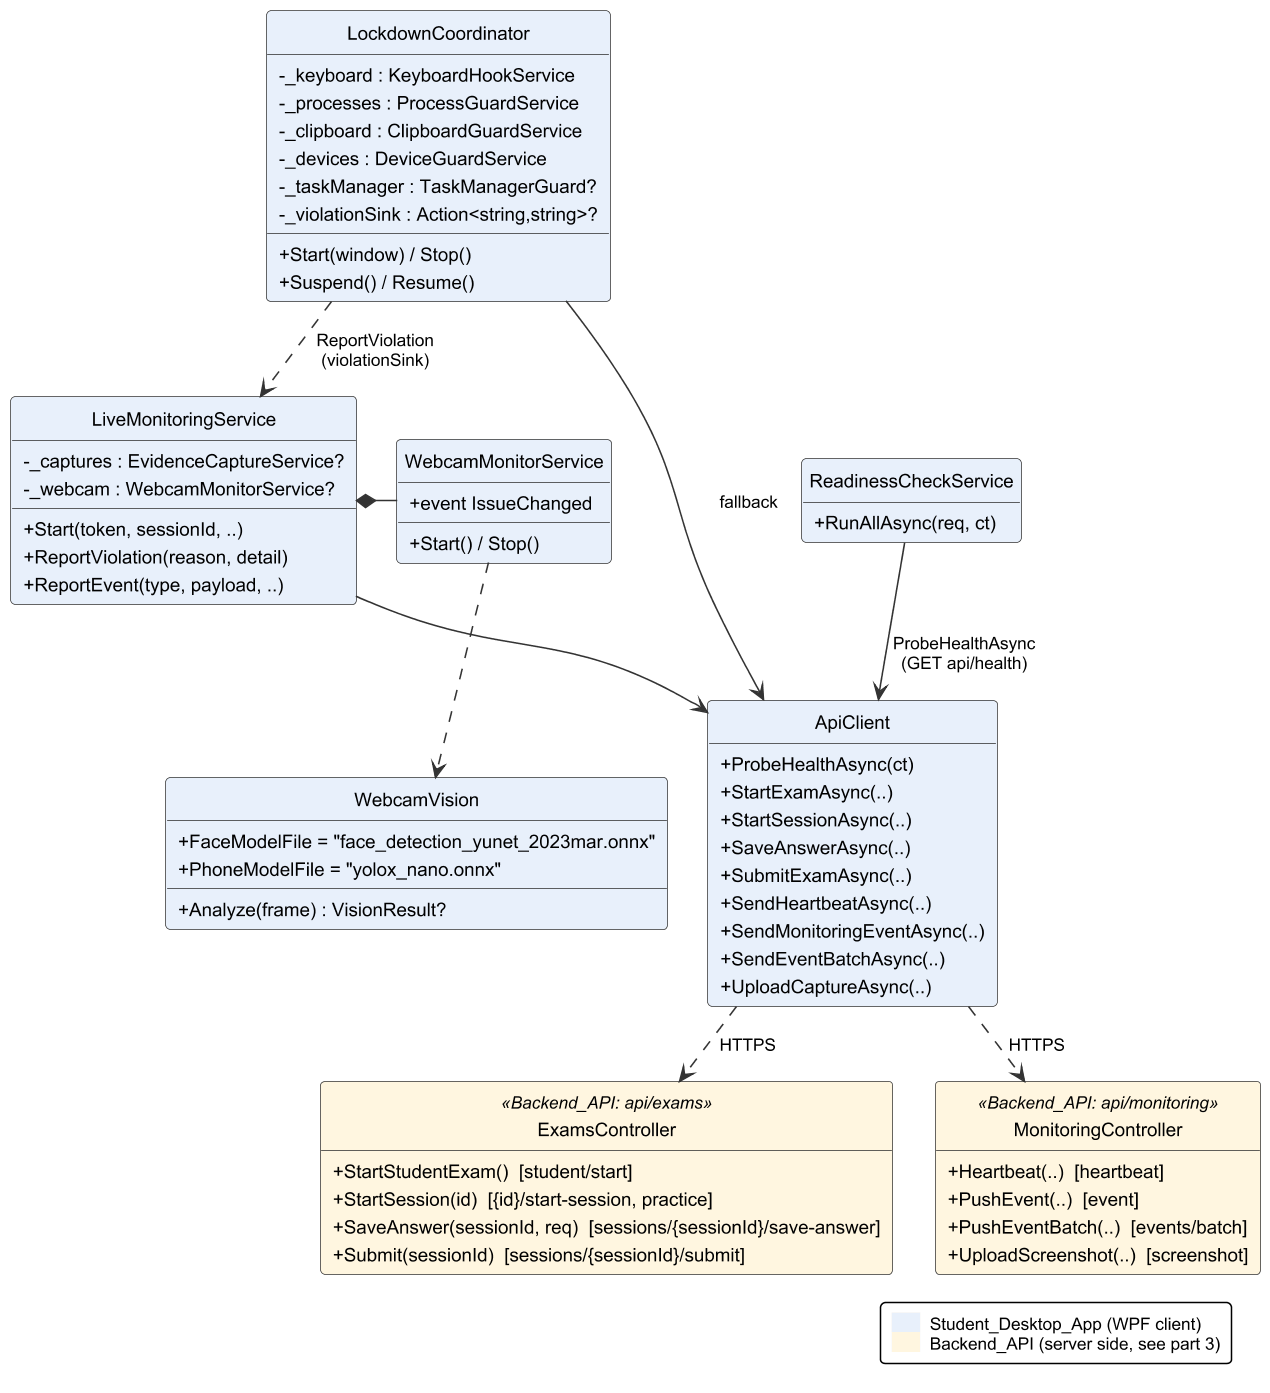
\includegraphics[width=0.85\linewidth]{Figures/class_diagram_client.png}
\caption{Class Diagram of the Student Desktop App Services}
\label{fig:class_diagram_client}
\end{figure}

\begin{figure}[!htbp]
\centering
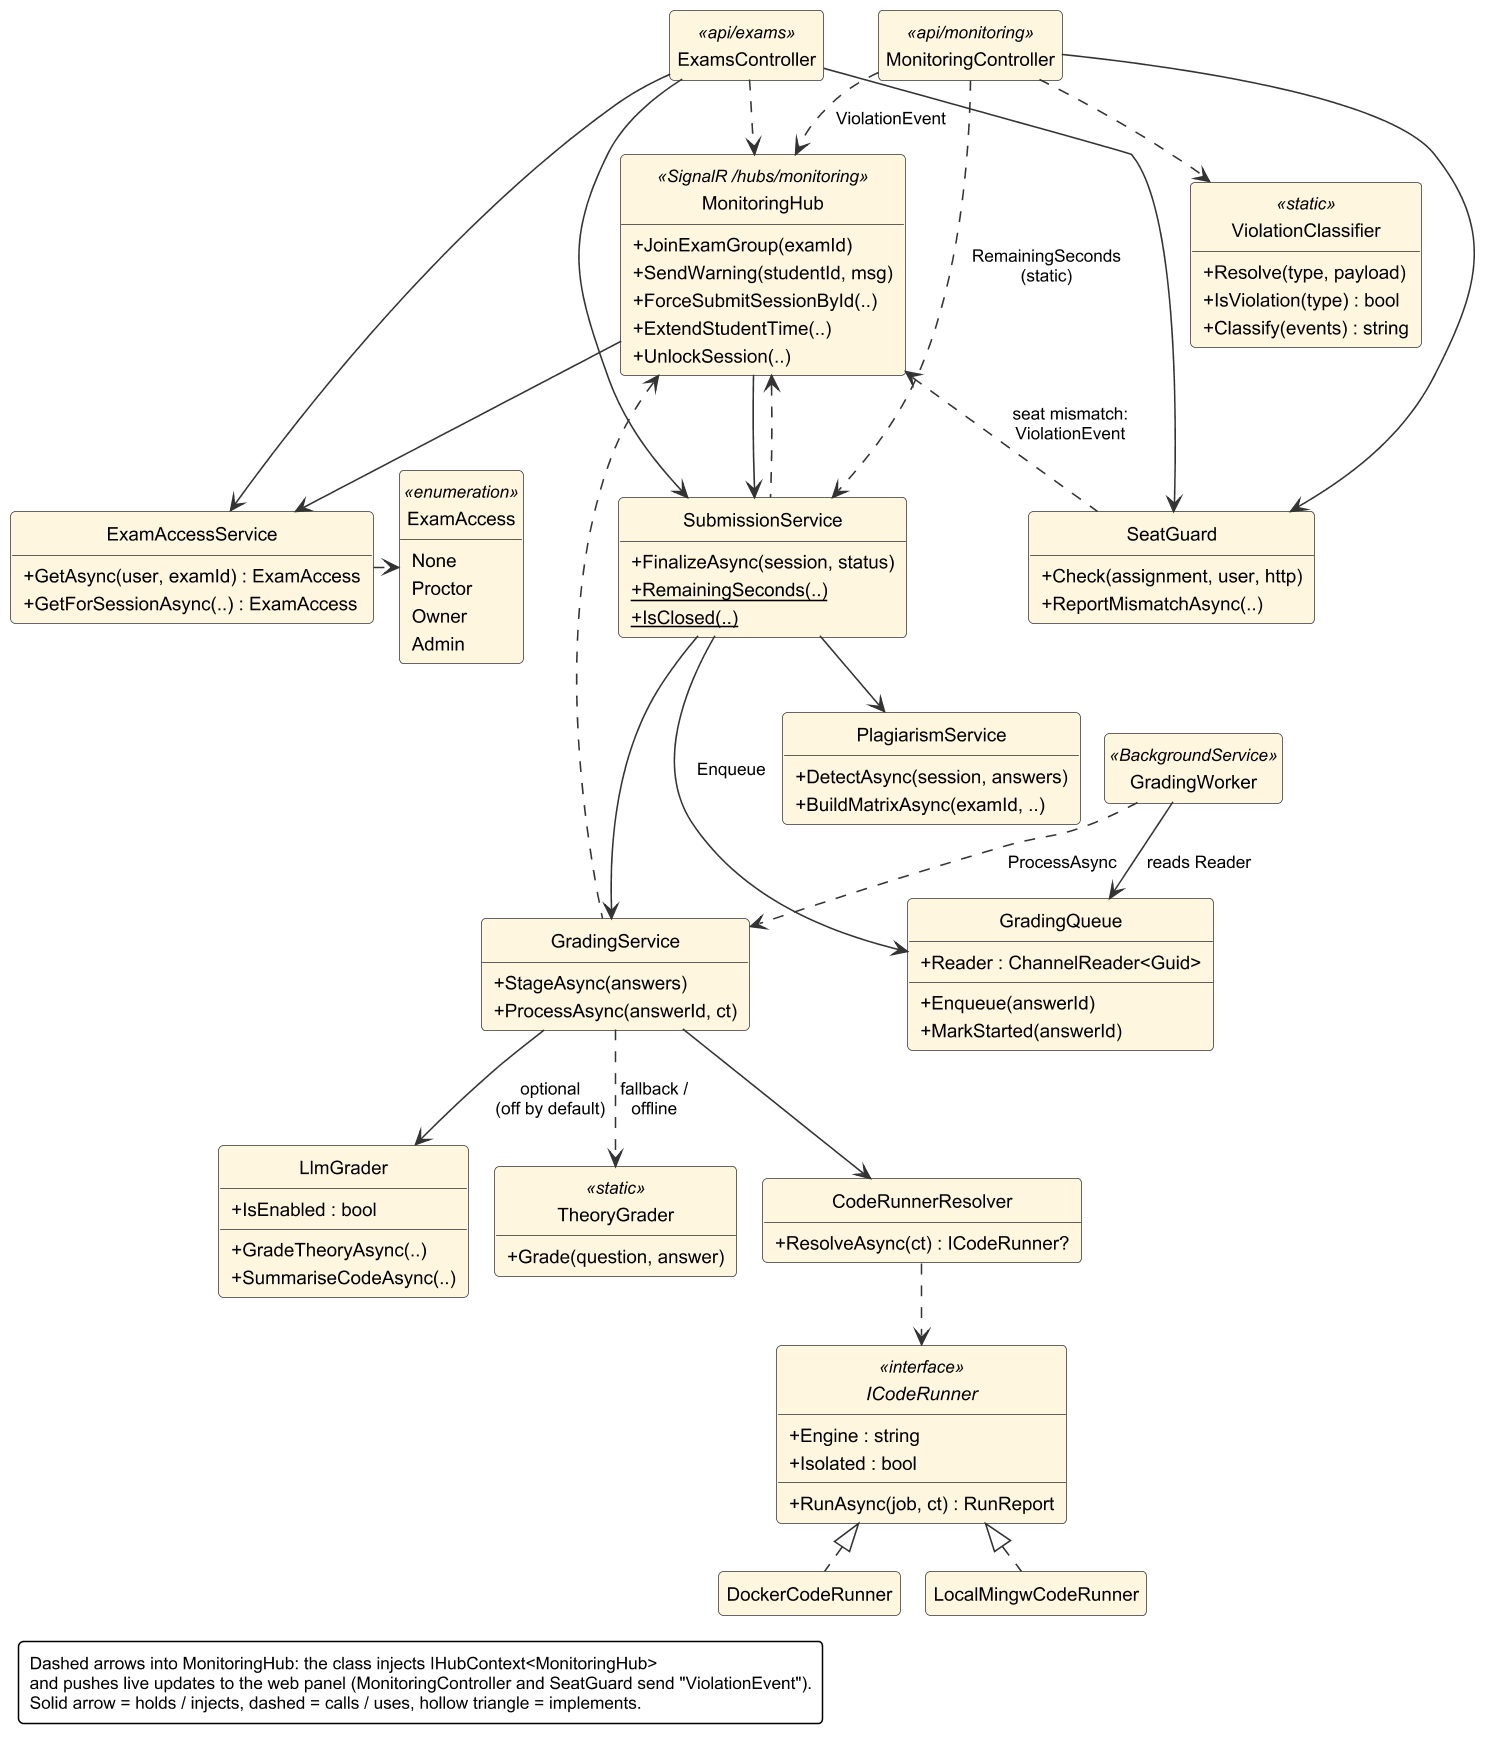
\includegraphics[width=\linewidth]{Figures/class_diagram_server.png}
\caption{Class Diagram of the Backend API Services}
\label{fig:class_diagram_server}
\end{figure}

\subsection{Deployment Diagram}
A deployment diagram maps software onto hardware nodes and network links \cite{deployment_diagram_vp}. Figure~\ref{fig:deployment_diagram} shows lab workstations running the WPF client with its ONNX models and encrypted outbox, browsers running the React panel, and a server running the ASP.NET Core~9 API, its SignalR hub (\url{/hubs/monitoring}), the hosted background services and a Docker \texttt{gcc:13} sandbox with a MinGW fallback. The server connects to Neon PostgreSQL, an SMTP server and, optionally, an LLM API. The desktop client uses REST only (plain HTTP on the shipped localhost configuration, HTTPS behind a TLS endpoint in deployment); the panel adds a SignalR connection for live updates.

\begin{figure}[!htbp]
\centering
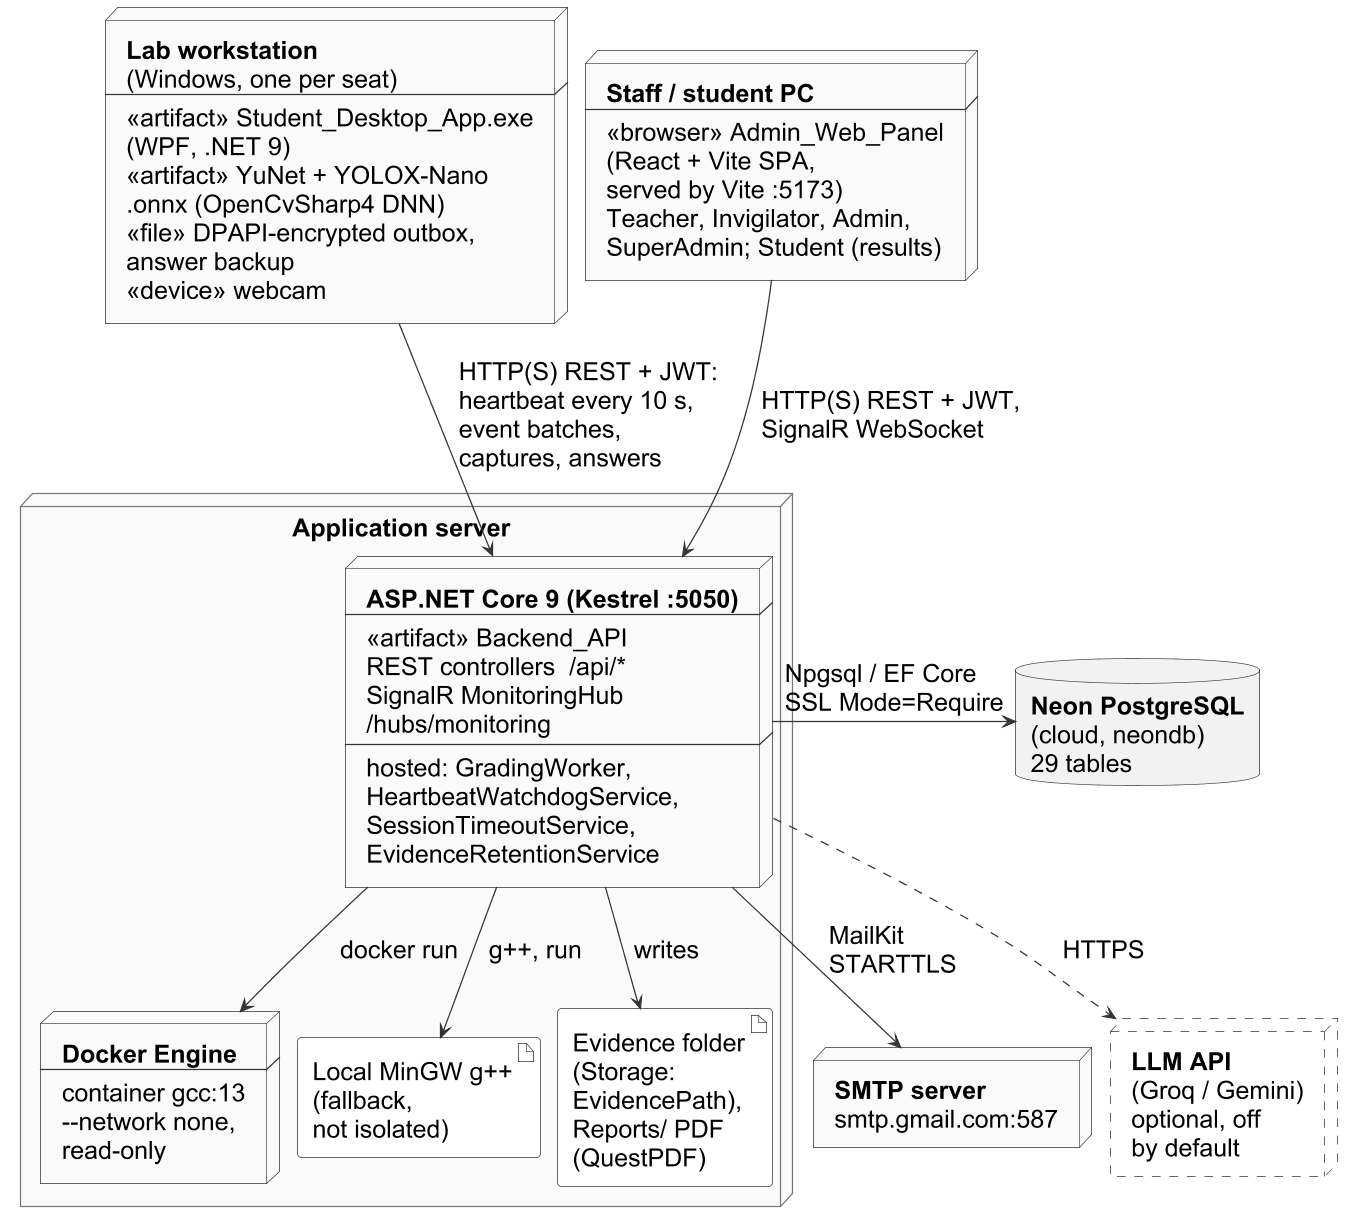
\includegraphics[width=0.97\linewidth]{Figures/deployment_diagram.png}
\caption{Deployment Diagram of SmartExam}
\label{fig:deployment_diagram}
\end{figure}

\subsection{Component Diagram}
Figure~\ref{fig:component_diagram} splits the system into client, server and data tiers. The server tier holds the 16 REST controllers, \texttt{MonitoringHub}, the domain services, hosted services such as \texttt{HeartbeatWatchdogService}, and the grading components. Submission triggers grading and plagiarism detection, and the Grading controller also calls the grading services directly.

\begin{figure}[!htbp]
\centering
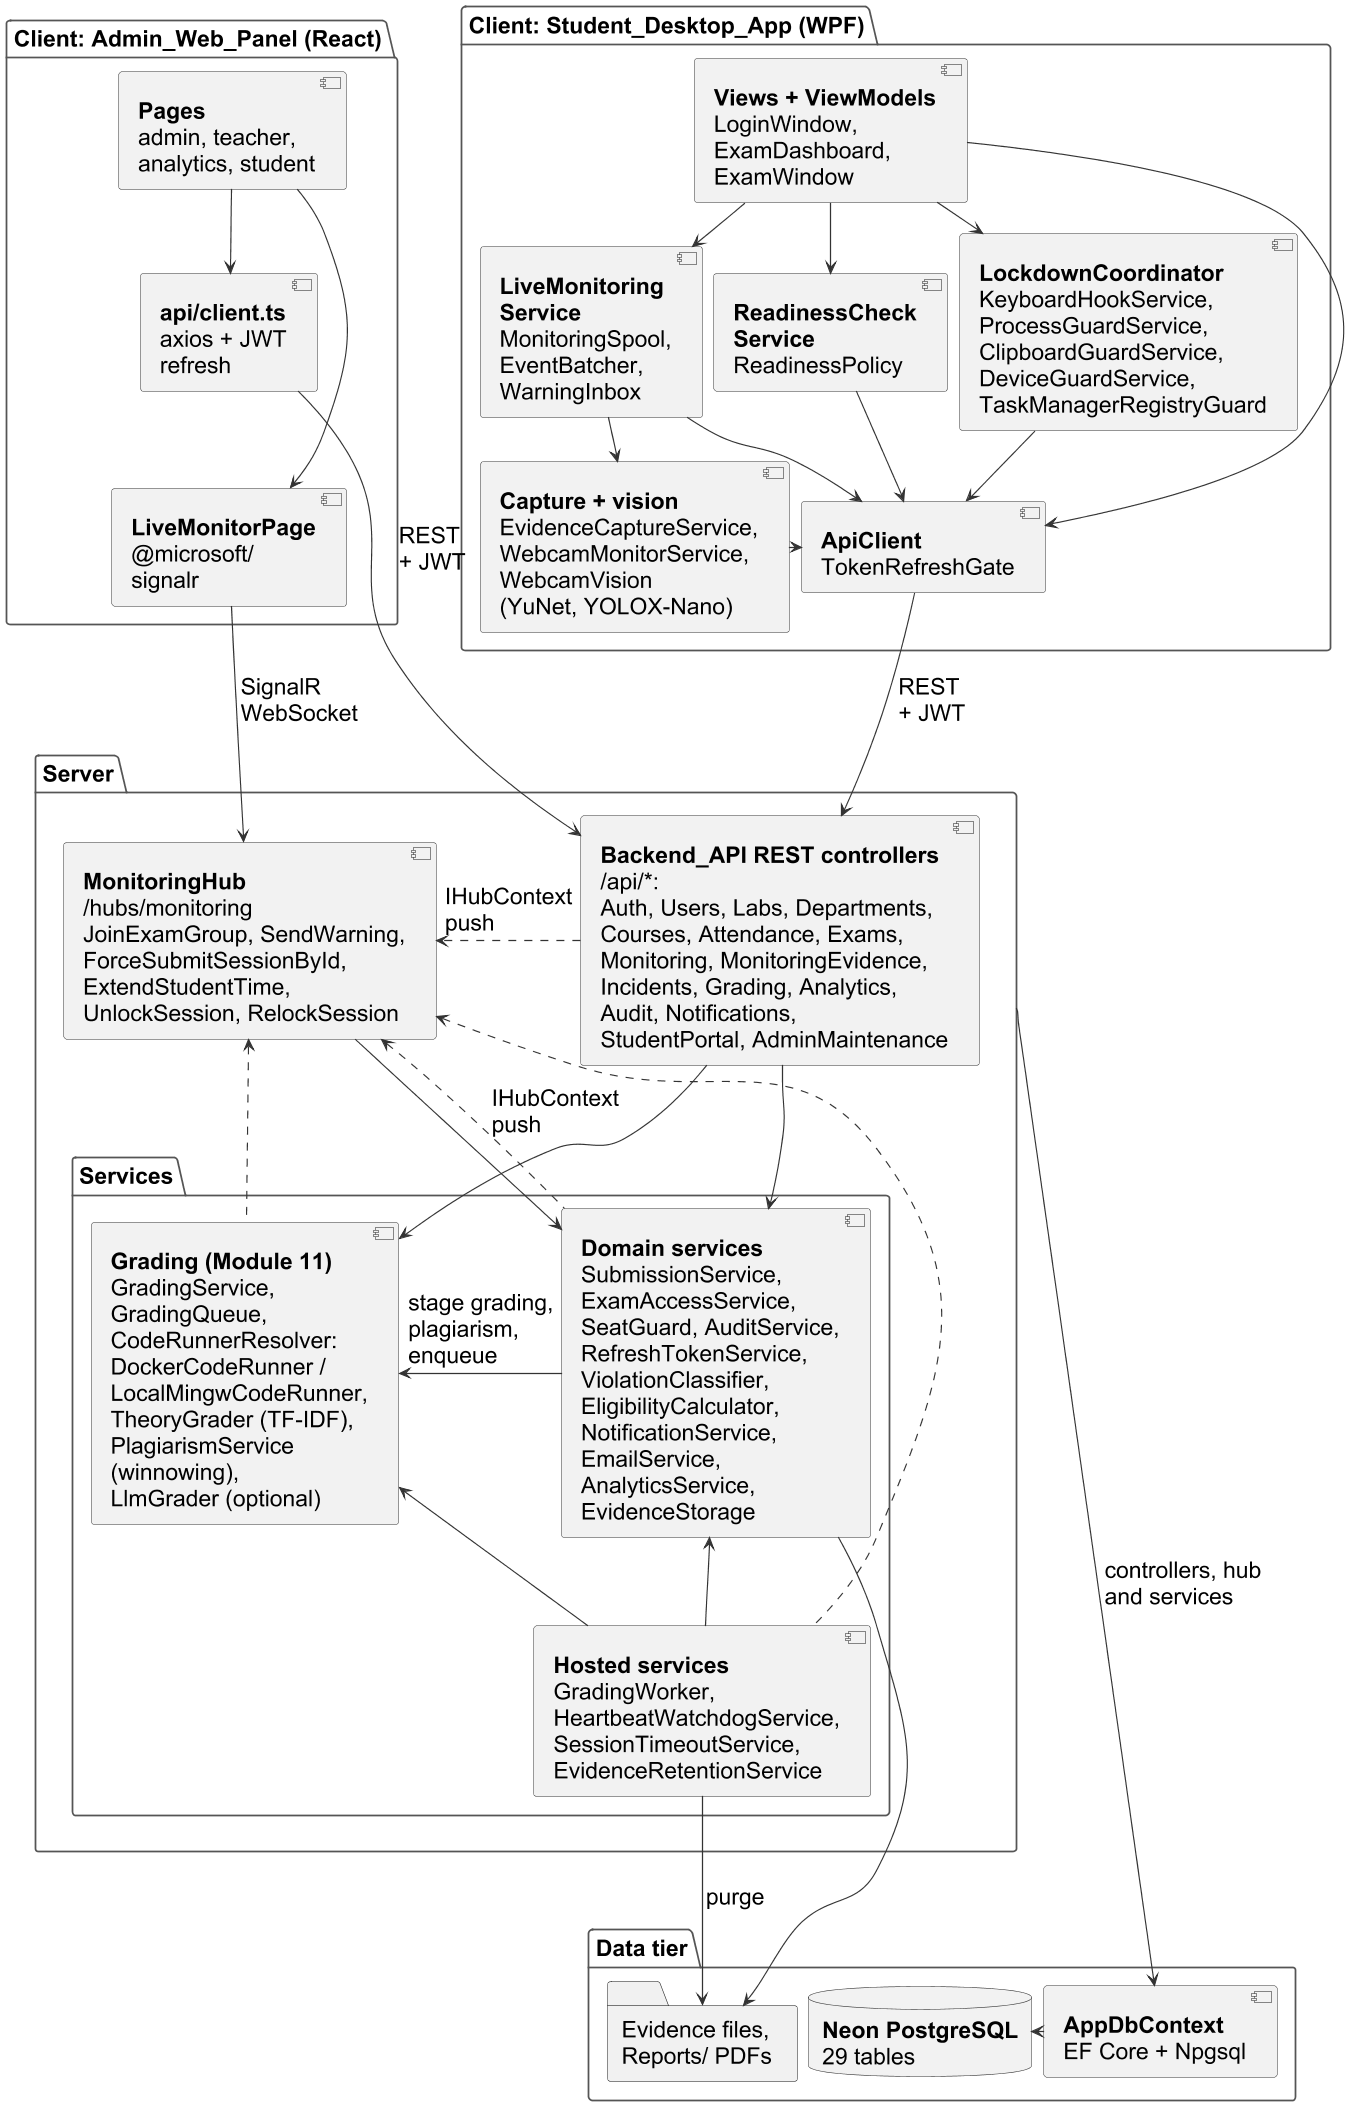
\includegraphics[width=0.92\linewidth]{Figures/component_diagram.png}
\caption{Component Diagram of SmartExam}
\label{fig:component_diagram}
\end{figure}

\section{Behavioural Diagrams}
Behavioural diagrams show run-time behaviour: steps, messages and state changes \cite{behavioral_uml_diagrams}.

\subsection{Activity Diagrams}
An activity diagram shows a workflow with its decisions and parallel branches \cite{activity_diagram_vp}. Figure~\ref{fig:activity_diagram} gives the whole student flow in Student, Desktop App, Server and Teacher swimlanes: login with the device check, readiness checks, the start gate, answering with lockdown and monitoring in parallel, then the end of the session by submit, timer, force-submit or timeout, followed by grading and teacher review.

\begin{figure}[!htbp]
\centering
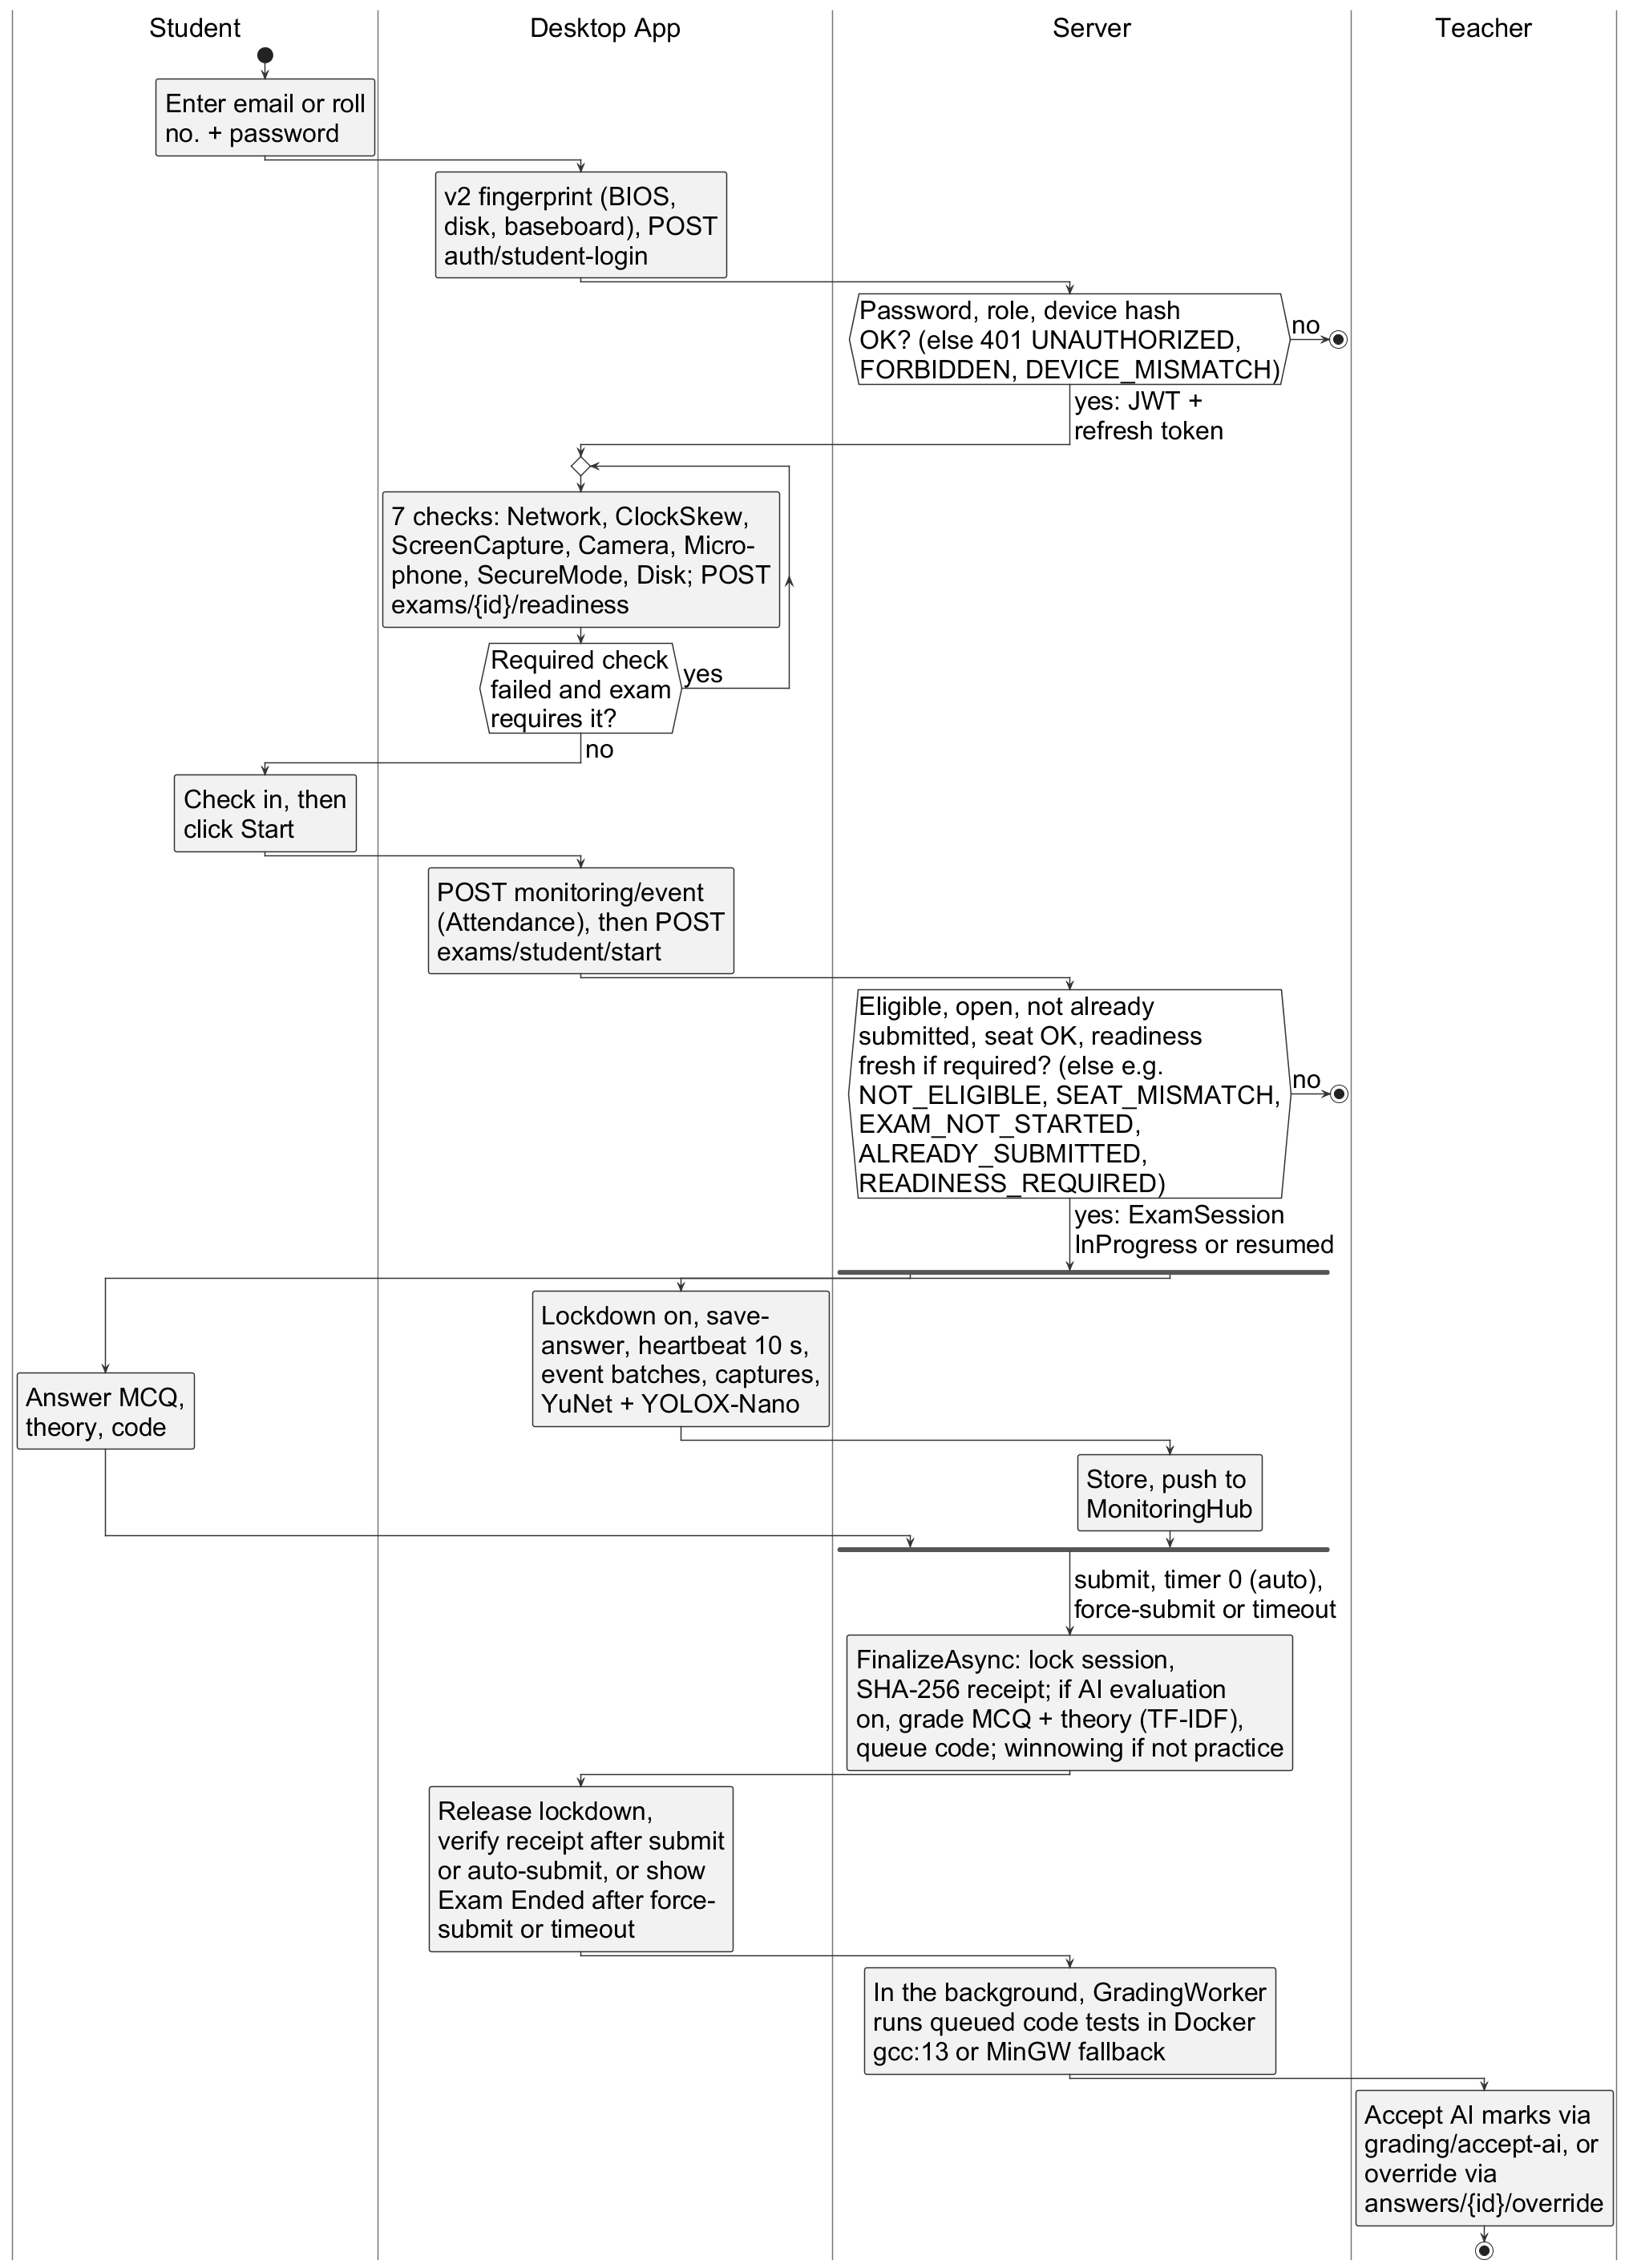
\includegraphics[width=\linewidth]{Figures/activity_diagram.png}
\caption{Activity Diagram of the Student Exam Session}
\label{fig:activity_diagram}
\end{figure}

\subsubsection{Login and Pre-Exam Checks}
In Figure~\ref{fig:activity_auth} the client sends the email or roll number, the password and a hardware fingerprint to \url{/api/auth/student-login}. The v2 fingerprint joins the BIOS, system-disk and baseboard serials read through WMI; the server stores only its SHA-256 hash. The first login saves the hash as the student's \texttt{DeviceBinding}, and a login from another machine is refused with \texttt{DEVICE\_MISMATCH}. Every outcome is audited, and a successful login returns a JWT and a refresh token.

Figure~\ref{fig:activity_diagnostics} shows the seven checks in \texttt{ReadinessPolicy}: network, clock skew, screen capture, webcam (one face, by YuNet) and microphone (when required), secure mode and disk space. Every run or retry posts all results to \url{/api/exams/{id}/readiness}, where the server recomputes the pass and pushes \texttt{ReadinessUpdated}. A pass is valid for 30 minutes, and Start unlocks once the exam opens.

\begin{figure}[!htbp]
\centering
\begin{minipage}[t]{0.48\linewidth}
\centering
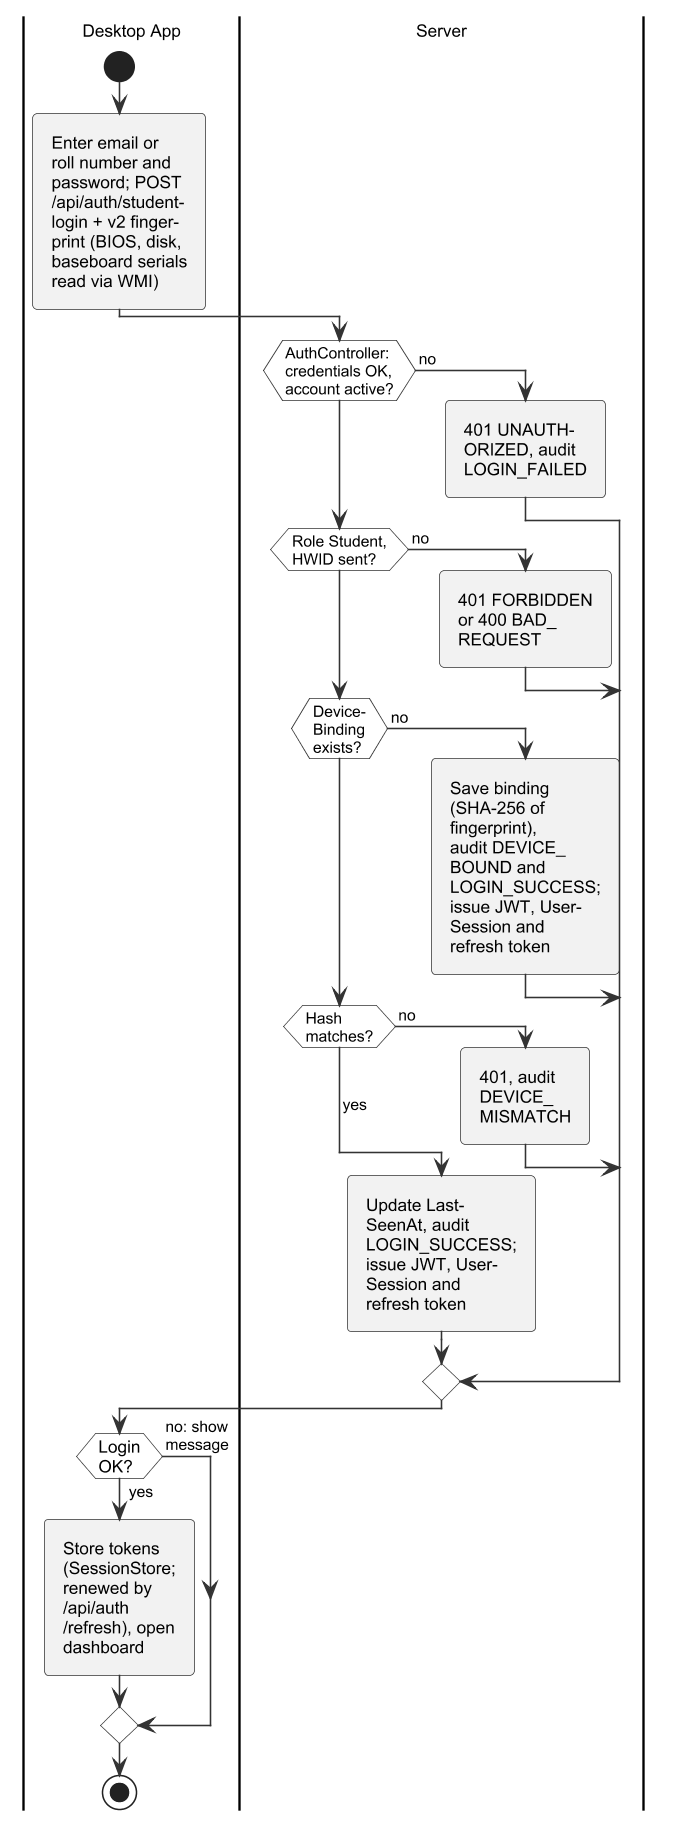
\includegraphics[width=\linewidth]{Figures/activity_auth.png}
\caption{Activity Diagram of Student Login and HWID Binding}
\label{fig:activity_auth}
\end{minipage}\hfill
\begin{minipage}[t]{0.48\linewidth}
\centering
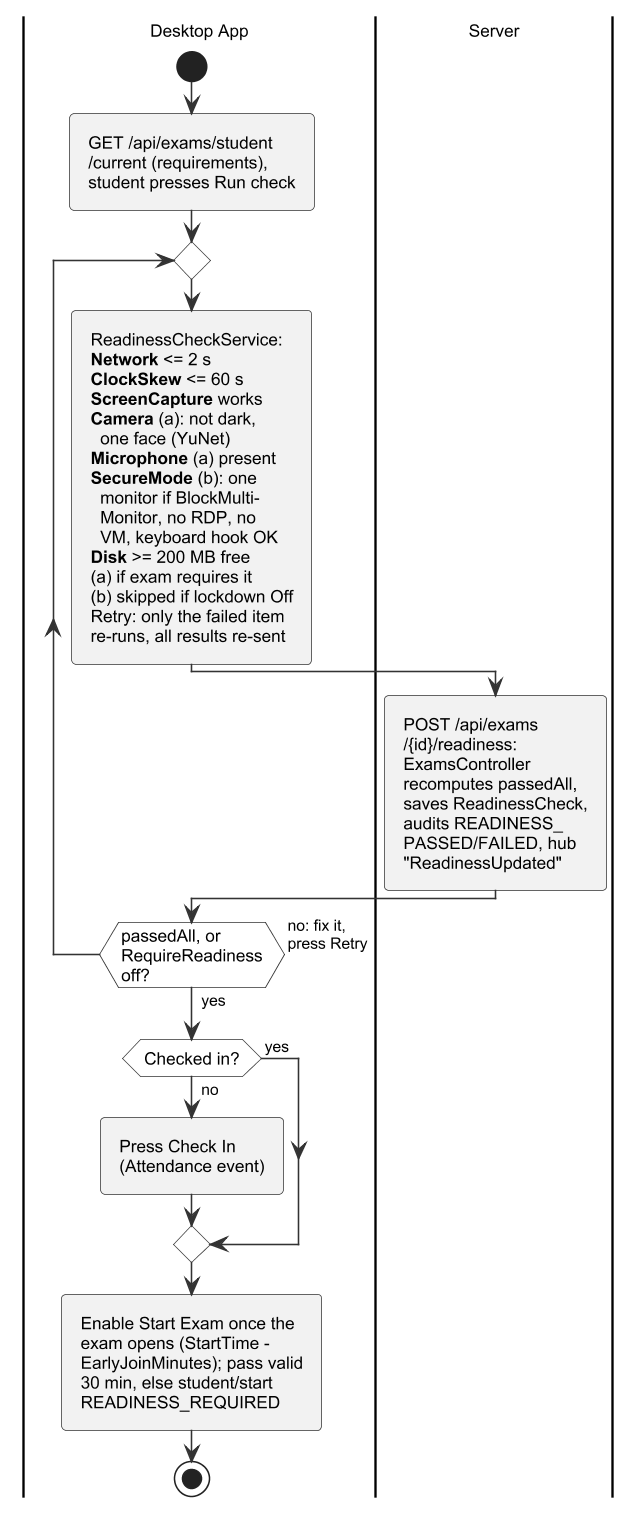
\includegraphics[width=\linewidth]{Figures/activity_diagnostics.png}
\caption{Activity Diagram of Pre-Exam Readiness Checks}
\label{fig:activity_diagnostics}
\end{minipage}
\end{figure}

\subsubsection{Mock Test and Exam Workspace}
\begin{sloppypar}
Practice exams (\texttt{Exam.IsMock}) are started through the normal \texttt{start-session} call and run in the same exam window, in Report mode and without the webcam, so students meet the editor and lockdown beforehand; they are graded but not checked for plagiarism (Figure~\ref{fig:activity_readiness}). During an exam (Figure~\ref{fig:activity_dashboard}) the window runs full screen under \texttt{LockdownCoordinator} and, when required, the webcam monitor. A blocked key, clipboard use, a disallowed app, a focus loss, a device violation or a webcam issue is spooled with a screenshot and sent to \url{/api/monitoring/events/batch}.
\end{sloppypar}

\begin{figure}[!htbp]
\centering
\begin{minipage}[t]{0.48\linewidth}
\centering
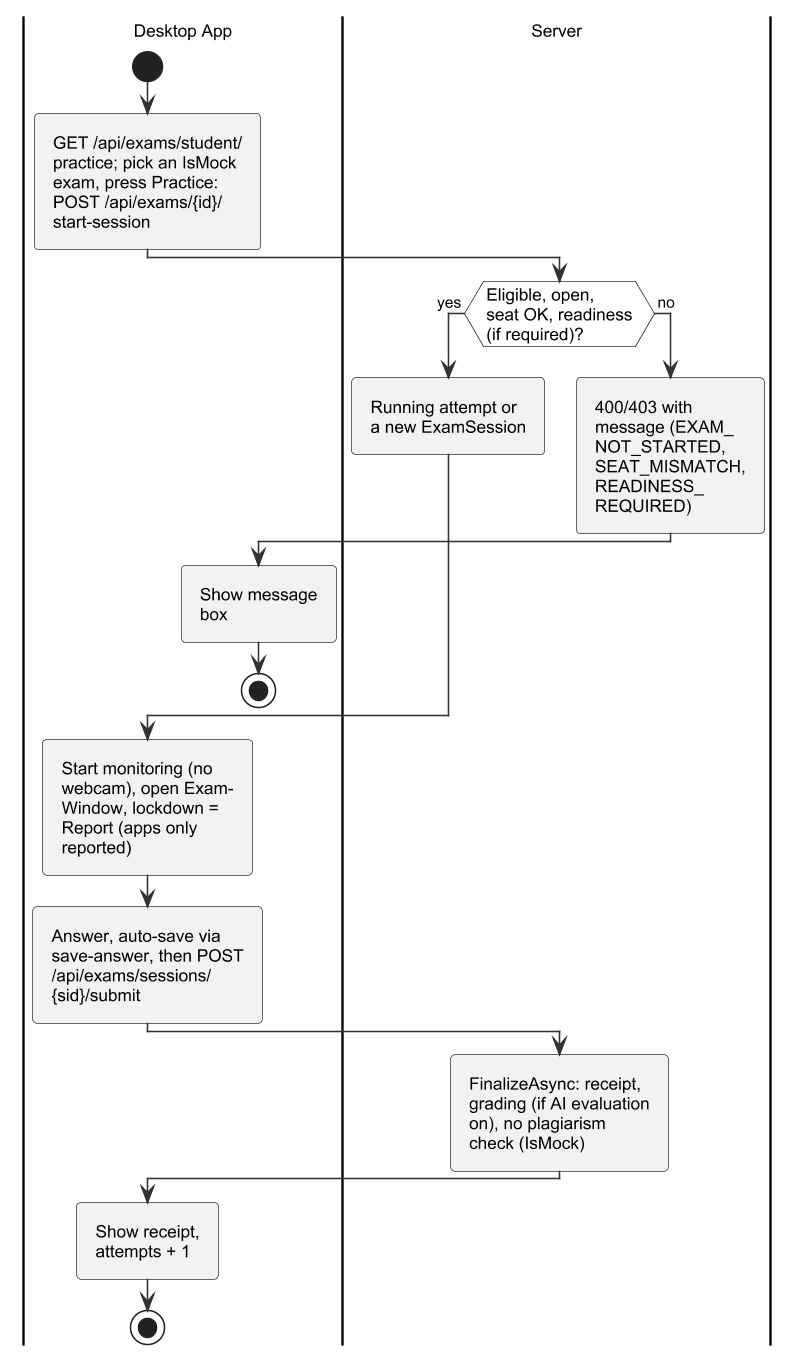
\includegraphics[width=\linewidth]{Figures/activity_readiness.png}
\caption{Activity Diagram of the Mock Test}
\label{fig:activity_readiness}
\end{minipage}\hfill
\begin{minipage}[t]{0.48\linewidth}
\centering
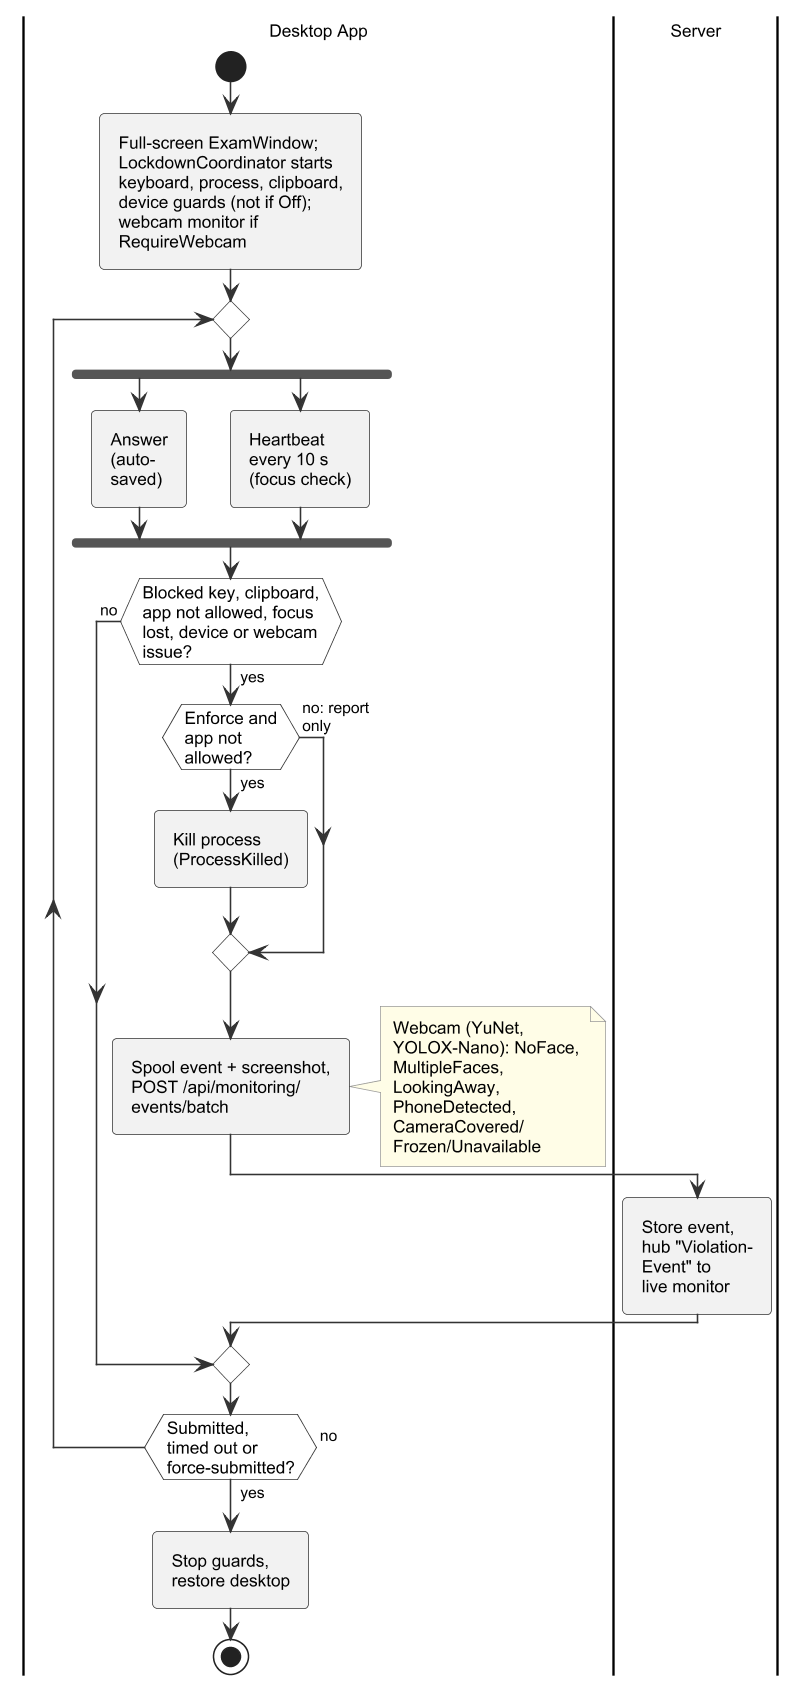
\includegraphics[width=\linewidth]{Figures/activity_dashboard.png}
\caption{Activity Diagram of the Active Exam Workspace}
\label{fig:activity_dashboard}
\end{minipage}
\end{figure}

\subsubsection{Auto-Save, Recovery and Submission}
An answer is saved 10 seconds after its first unsaved edit, on question change and on focus loss. Every edit also goes to a local AES-256-GCM backup whose key is protected by DPAPI. Failed saves are queued and replayed when the network returns, and a restarted client merges the backup with the server copy (Figure~\ref{fig:activity_recovery}).

On submit or timer expiry (Figure~\ref{fig:activity_submission}) the client flushes pending saves; if any answer is still unsent it keeps the window open and retries every 10 seconds. Otherwise it submits, and \texttt{FinalizeAsync} sets the session to Submitted with a SHA-256 receipt, which the client verifies. \texttt{SessionTimeoutService} finalises overdue sessions as TimedOut.

\begin{figure}[!htbp]
\centering
\begin{minipage}[t]{0.48\linewidth}
\centering
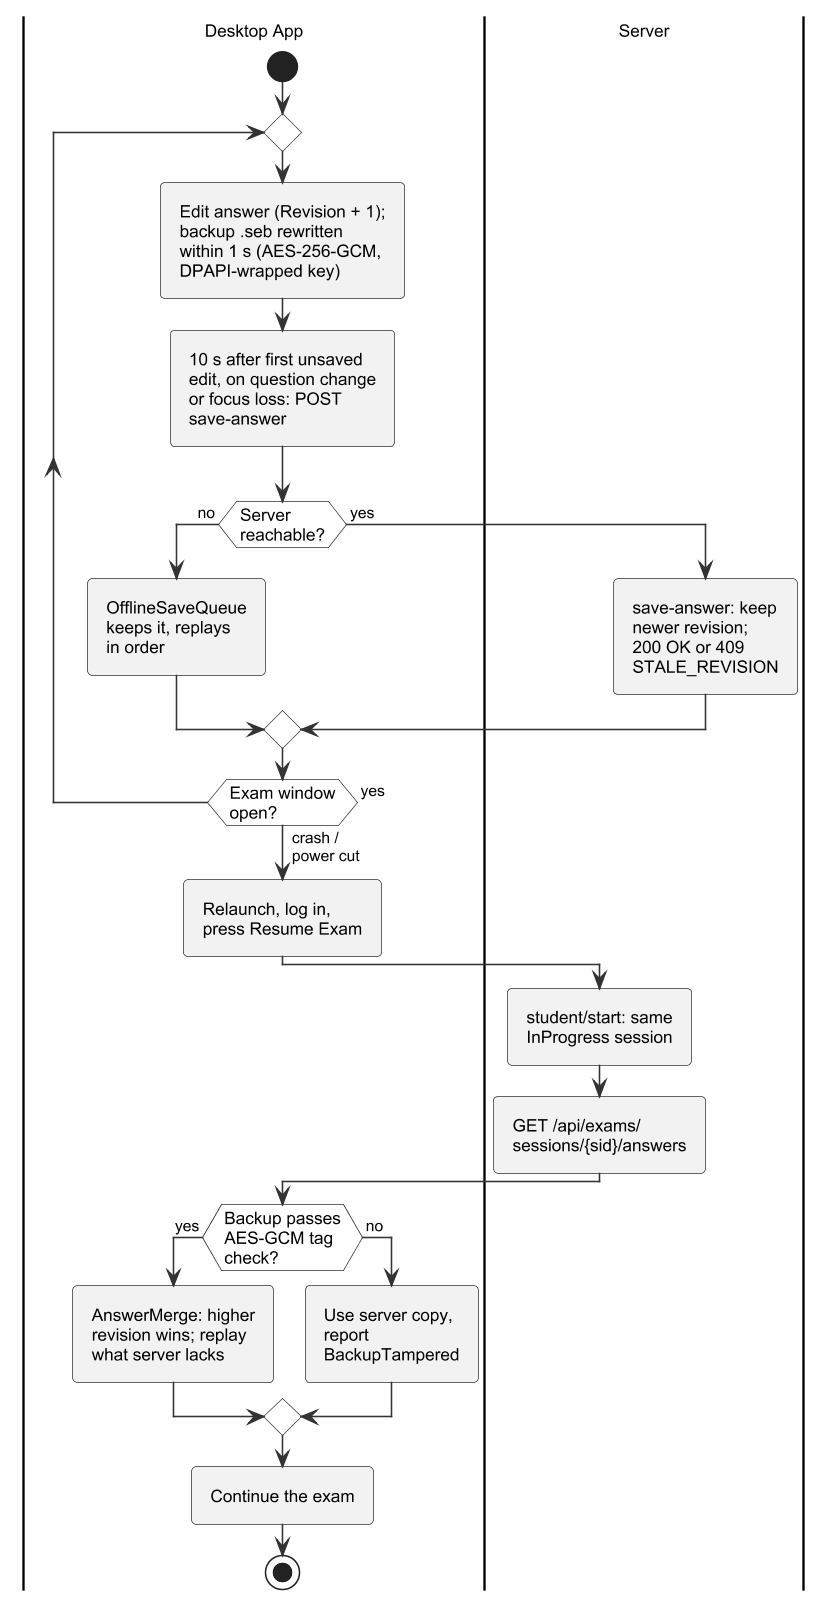
\includegraphics[width=\linewidth]{Figures/activity_recovery.png}
\caption{Activity Diagram of Auto-Save and Session Recovery}
\label{fig:activity_recovery}
\end{minipage}\hfill
\begin{minipage}[t]{0.48\linewidth}
\centering
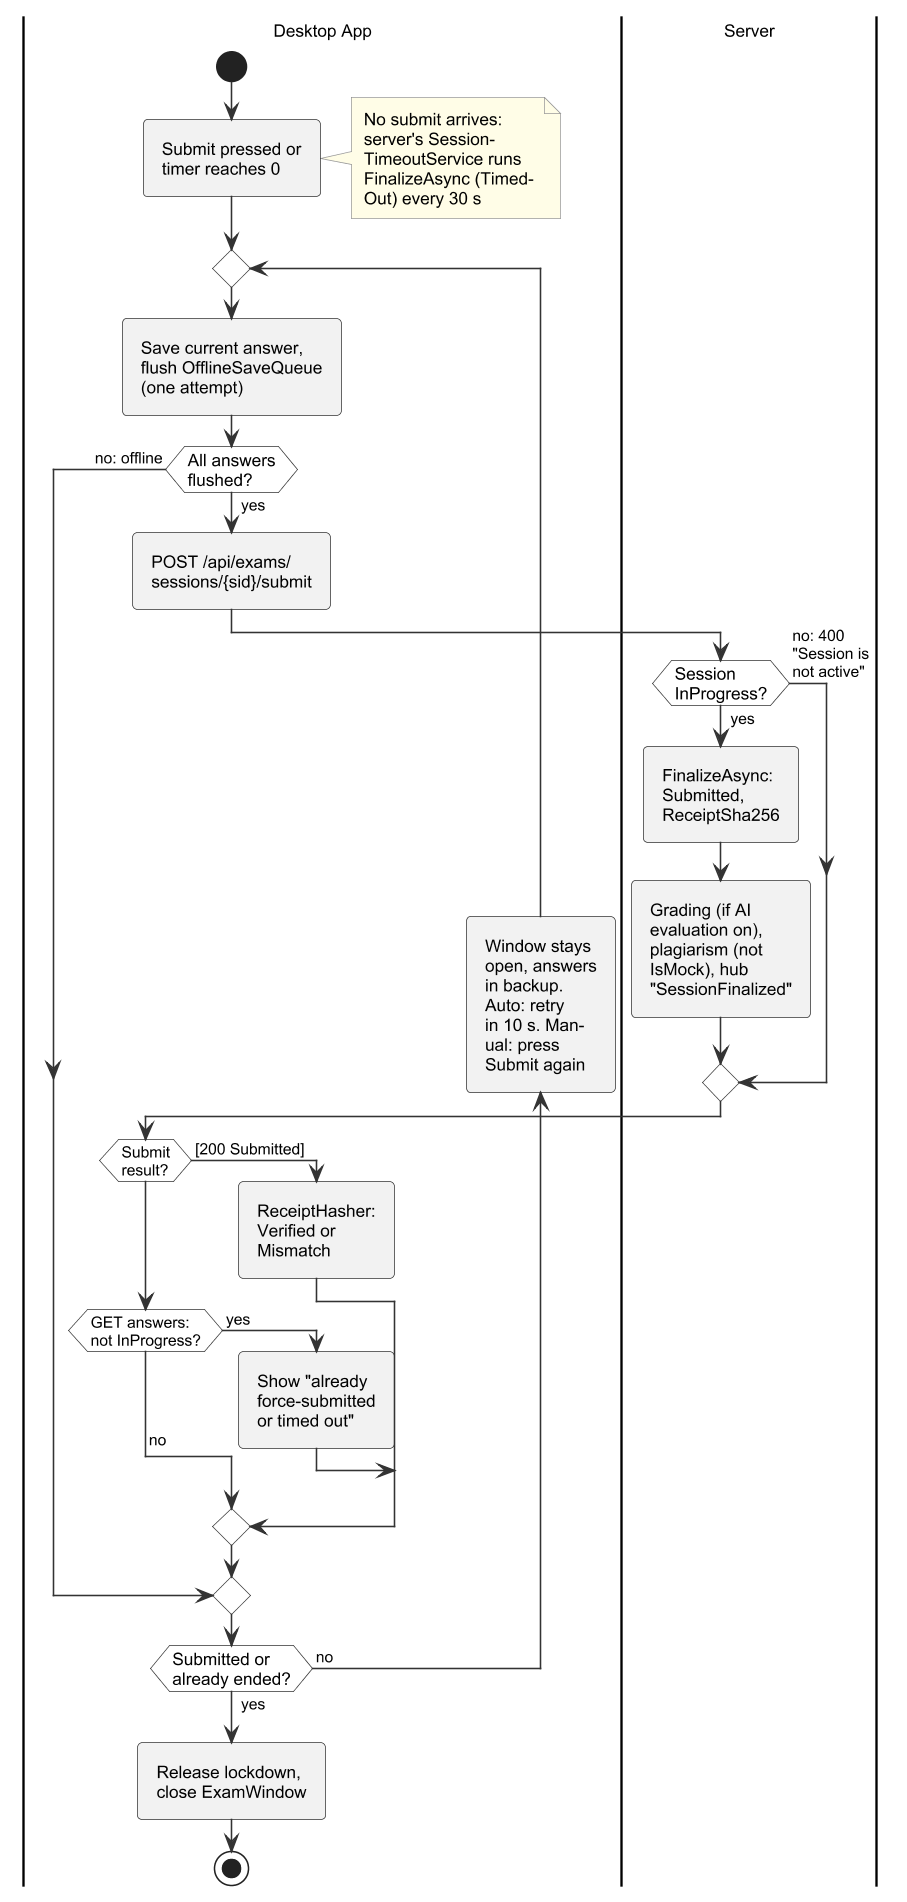
\includegraphics[width=\linewidth]{Figures/activity_submission.png}
\caption{Activity Diagram of Exam Submission}
\label{fig:activity_submission}
\end{minipage}
\end{figure}

\subsubsection{Exam Configuration}
A teacher fills a four-step wizard (basic info, questions, rules, students) to create or edit an exam (Figure~\ref{fig:activity_config}). \texttt{ExamsController} validates the payload, for example requiring a test case for every coding question, and refuses students outside the teacher's sections; an exam can be edited only while it is Scheduled. Allowed applications are stored as a JSON list of executable names in \texttt{Exam.AllowedApps} (Figure~\ref{fig:activity_applications}). \texttt{ProcessGuardService} scans every 2 seconds; in Enforce mode it kills a disallowed process tree (\texttt{ProcessKilled}), and in Report mode it only reports it (\texttt{UnauthorizedProcess}).

\begin{figure}[!htbp]
\centering
\begin{minipage}[t]{0.48\linewidth}
\centering
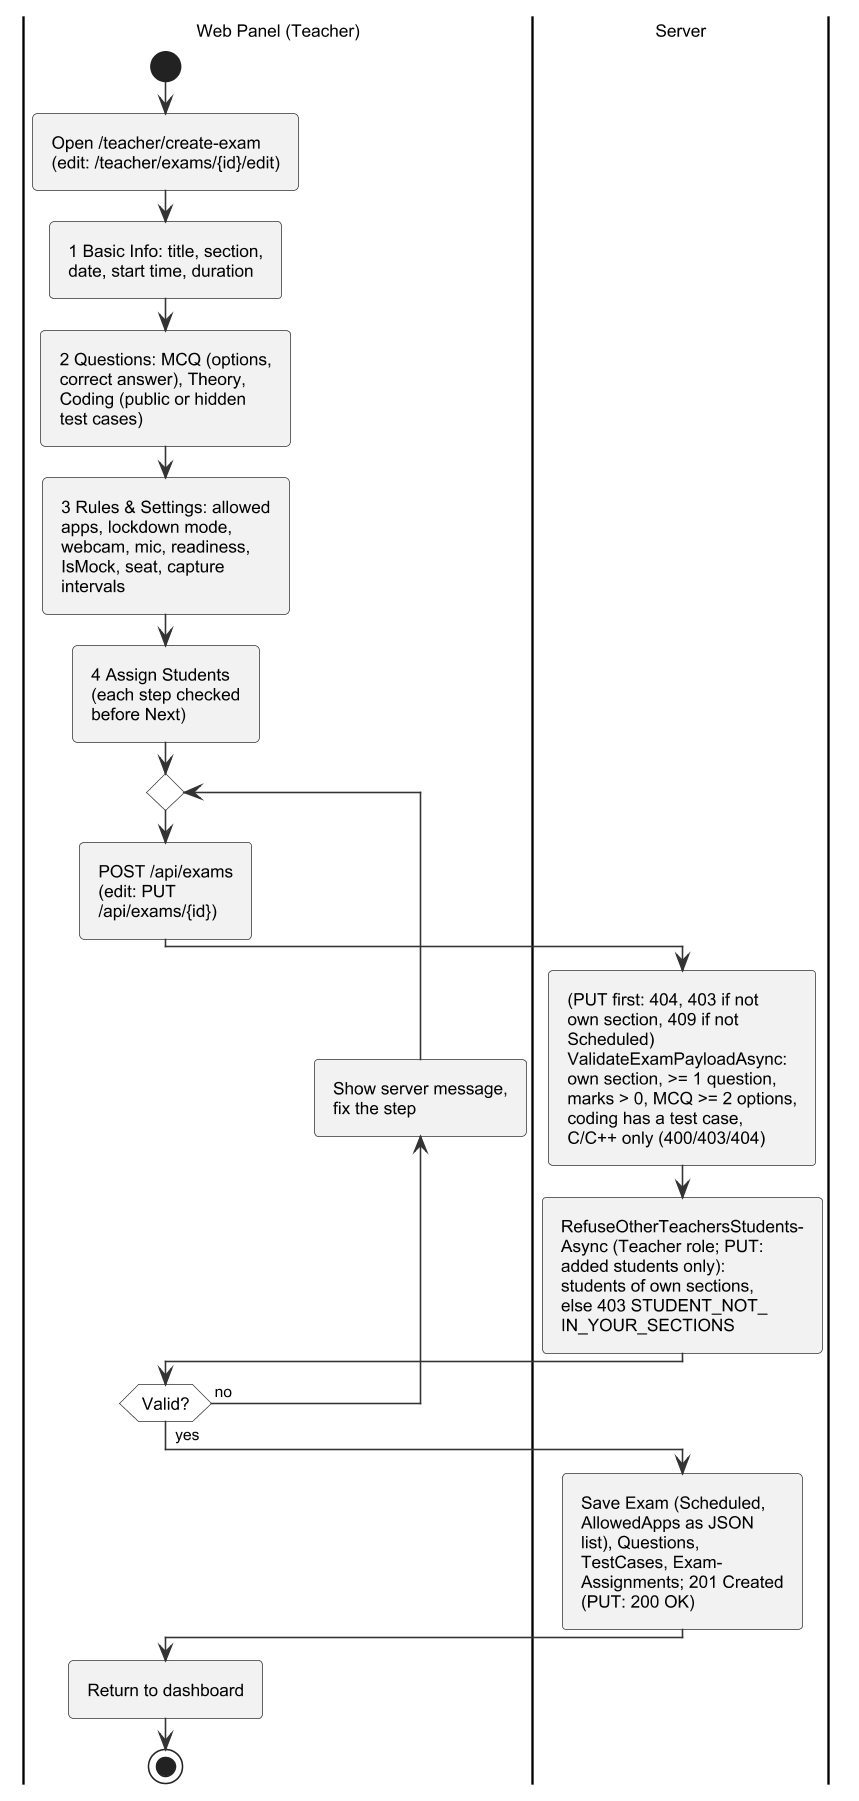
\includegraphics[width=\linewidth]{Figures/activity_config.png}
\caption{Activity Diagram of Exam Configuration}
\label{fig:activity_config}
\end{minipage}\hfill
\begin{minipage}[t]{0.48\linewidth}
\centering
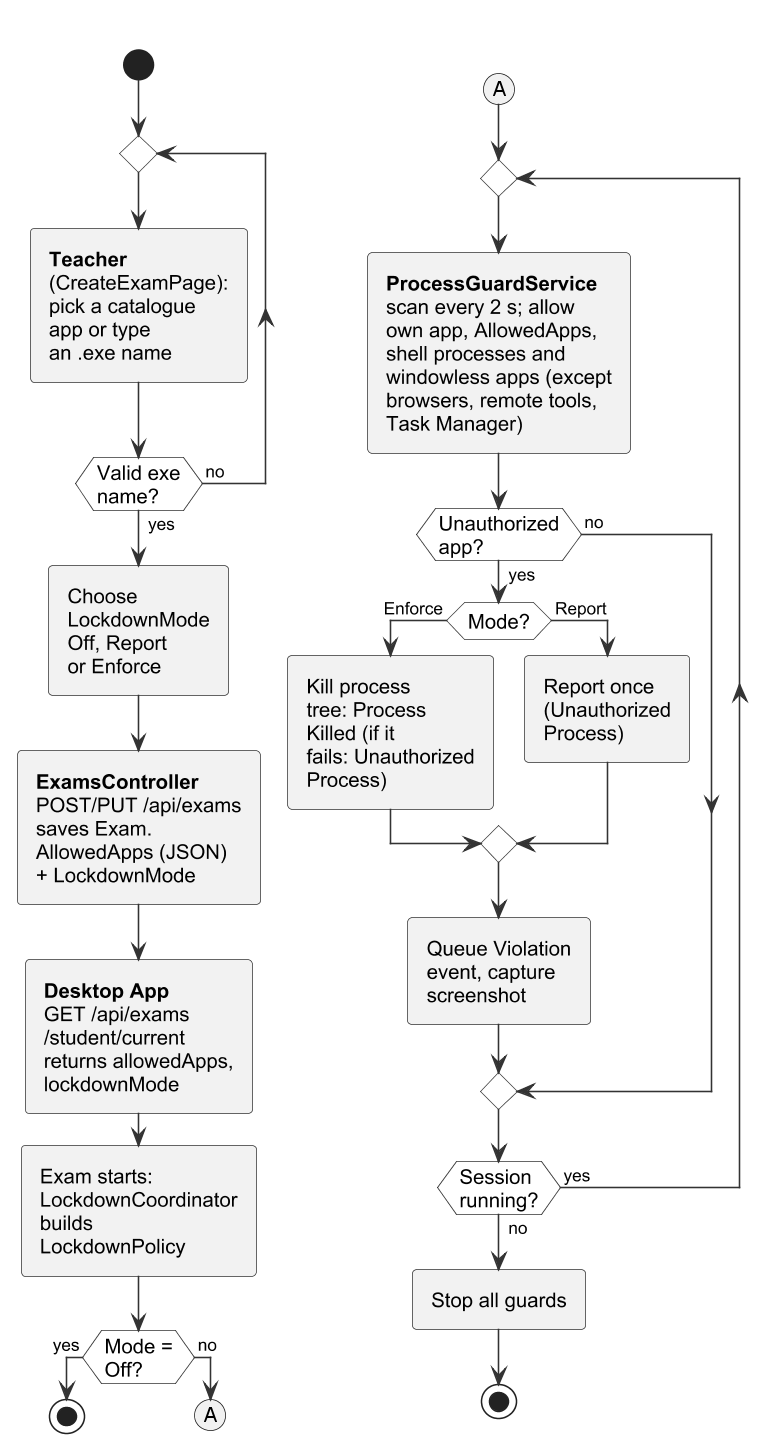
\includegraphics[width=\linewidth]{Figures/activity_applications.png}
\caption{Activity Diagram of Allowed Applications Configuration}
\label{fig:activity_applications}
\end{minipage}
\end{figure}

\subsubsection{Seating and Live Monitoring}
\begin{sloppypar}
Admins register lab workstations (machine number, host name, IP address), and the teacher assigns one to each student on the Eligibility page (Figure~\ref{fig:activity_seating}). A start from a non-desktop token is refused with \texttt{DESKTOP\_CLIENT\_REQUIRED}. When \texttt{Exam.EnforceSeat} is on, \texttt{SeatGuard} compares the machine name or IP with the assigned seat; a mismatch blocks the start with \texttt{SEAT\_MISMATCH} and alerts the proctors, and each heartbeat re-checks the seat.
\end{sloppypar}

\begin{sloppypar}
In Figure~\ref{fig:activity_monitoring} the live monitor page joins the exam's group on \texttt{MonitoringHub}. Clients send heartbeats, event batches and screenshots over REST to \texttt{MonitoringController}, which stores them and pushes them to the page. Staff can warn a student, extend their time or force-submit, and the client learns the result from its next heartbeat reply. \texttt{HeartbeatWatchdogService} marks a session disconnected after 30 seconds without a heartbeat.
\end{sloppypar}

\begin{figure}[!htbp]
\centering
\begin{minipage}[t]{0.48\linewidth}
\centering
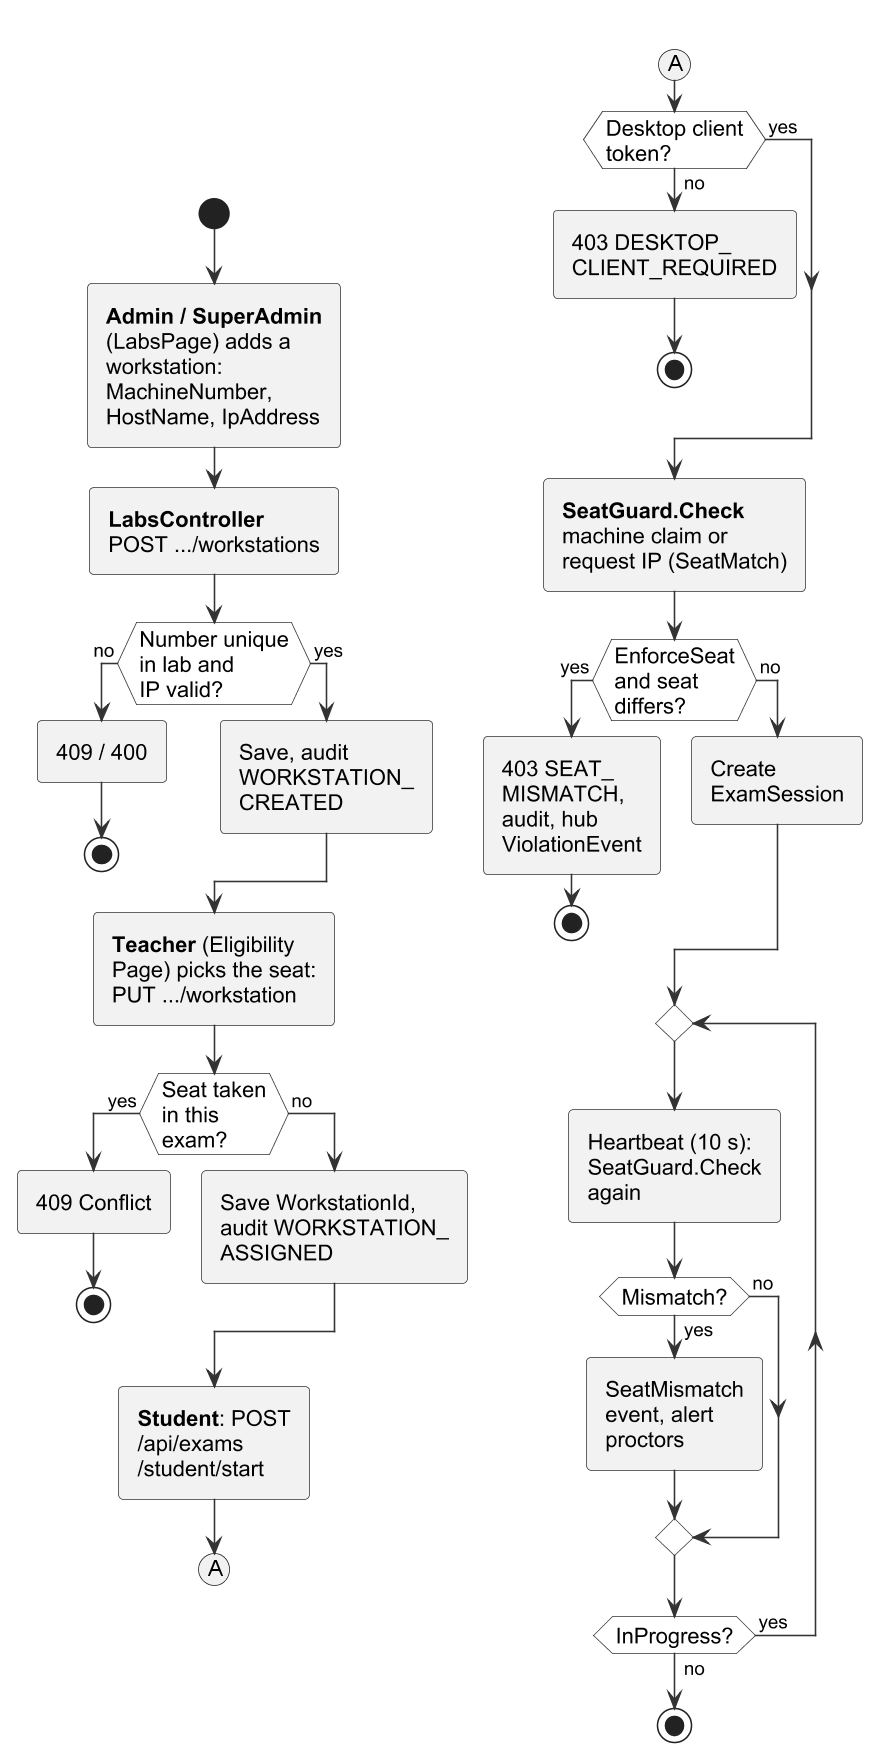
\includegraphics[width=\linewidth]{Figures/activity_seating.png}
\caption{Activity Diagram of Seat Assignment}
\label{fig:activity_seating}
\end{minipage}\hfill
\begin{minipage}[t]{0.48\linewidth}
\centering
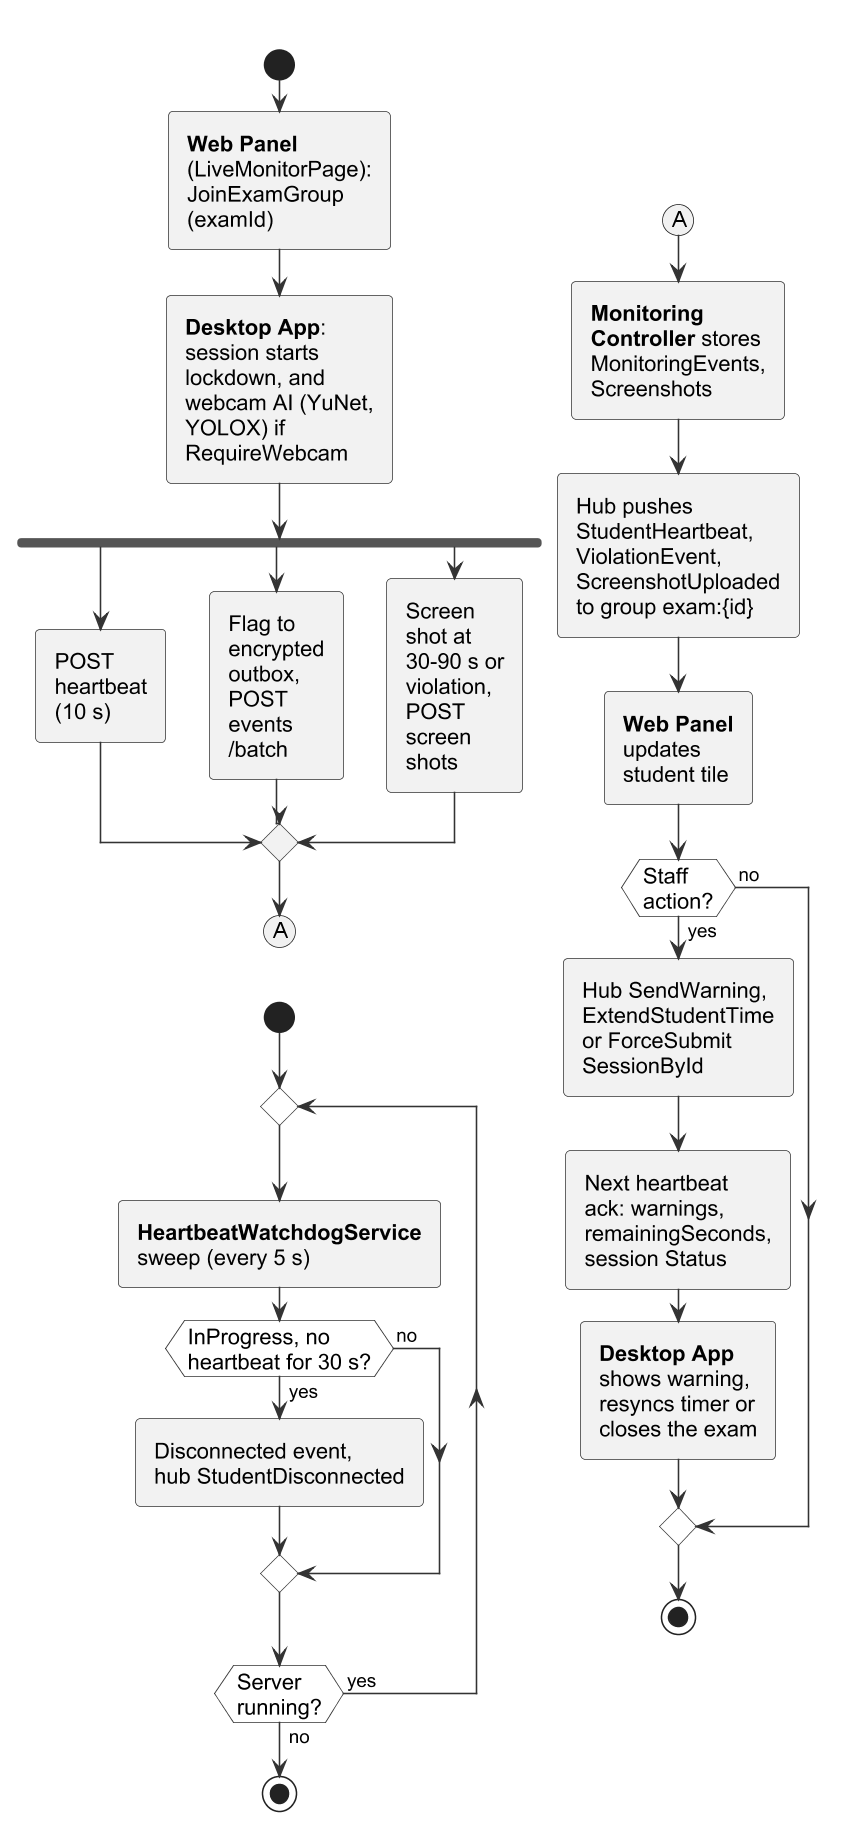
\includegraphics[width=\linewidth]{Figures/activity_monitoring.png}
\caption{Activity Diagram of Live Monitoring}
\label{fig:activity_monitoring}
\end{minipage}
\end{figure}

\subsubsection{Grading, Reports and Audit}
After submission (Figure~\ref{fig:activity_grading}) MCQ answers are checked against the key, and theory answers are scored by TF-IDF (0.7 cosine similarity plus 0.3 key-term coverage) or queued for the optional LLM grader. Plagiarism is checked pairwise with k-gram winnowing for non-practice exams. \texttt{GradingWorker} then runs each coding answer against its test cases in Docker \texttt{gcc:13} (no network) or the MinGW fallback; without a runner the answer is left for teacher review. The teacher can accept or override every suggested mark.

\begin{figure}[!htbp]
\centering
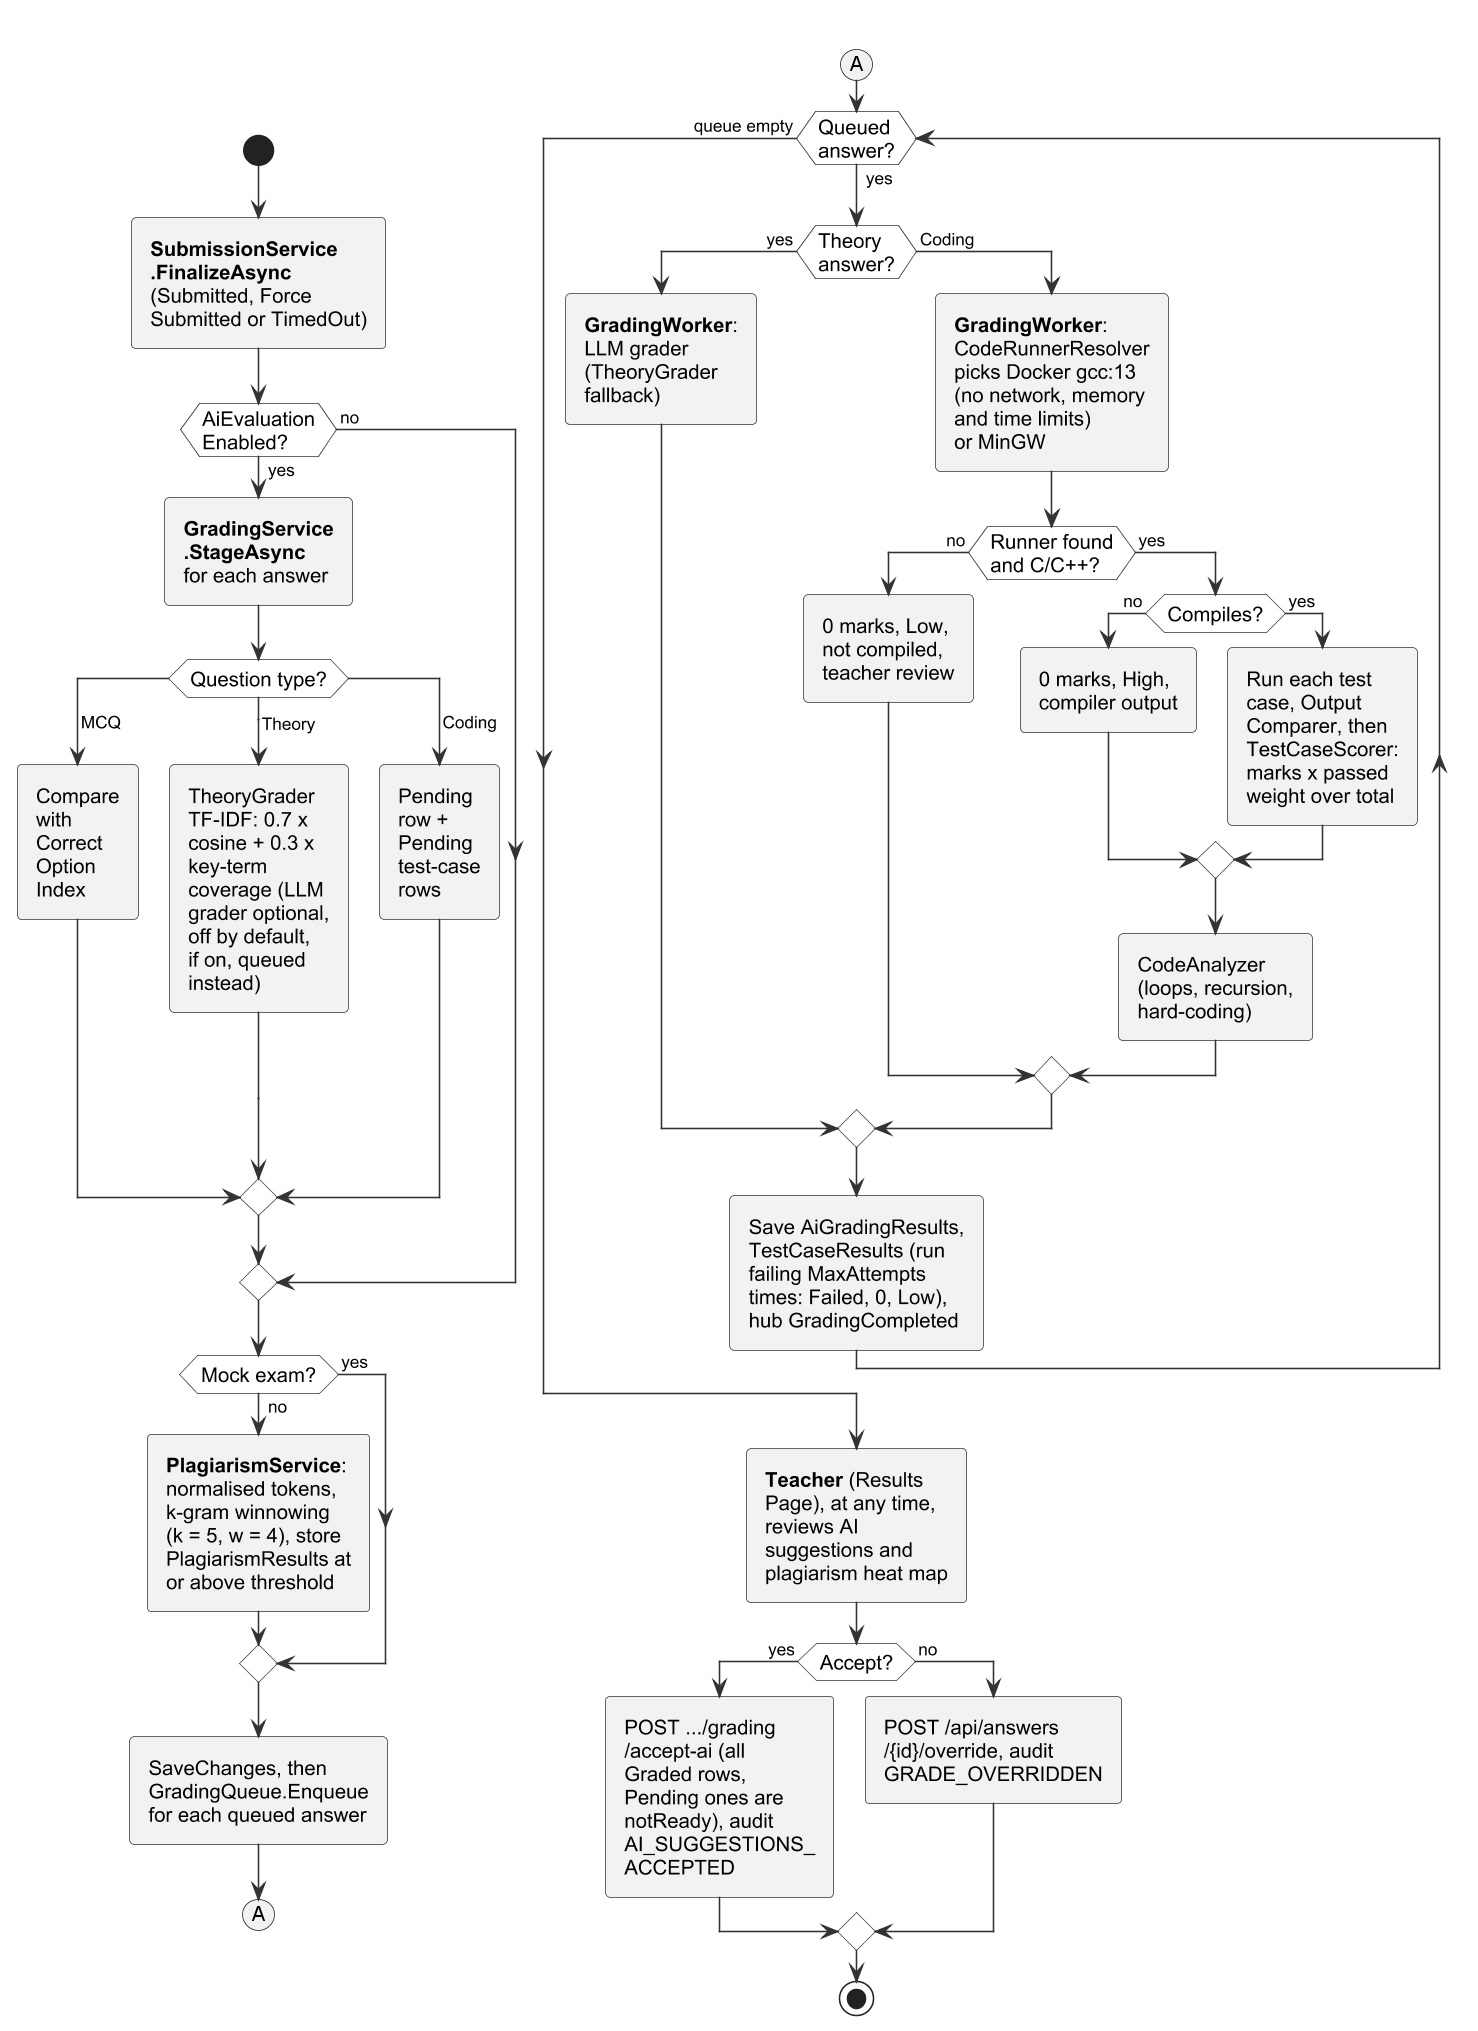
\includegraphics[width=0.8\linewidth]{Figures/activity_grading.png}
\caption{Activity Diagram of AI-Assisted Grading and Plagiarism Check}
\label{fig:activity_grading}
\end{figure}

For a report (Figure~\ref{fig:activity_report}) the API renders a QuestPDF document with summary statistics, per-question performance and the score distribution, records it in \texttt{ExamReports} and returns a download link; report generation is not audited. Controllers write audit entries explicitly through \texttt{AuditService}, saving refused actions at once and staging others with the change they record, and admins read them on the audit page (Figure~\ref{fig:activity_audit}).

\begin{figure}[!htbp]
\centering
\begin{minipage}[t]{0.48\linewidth}
\centering
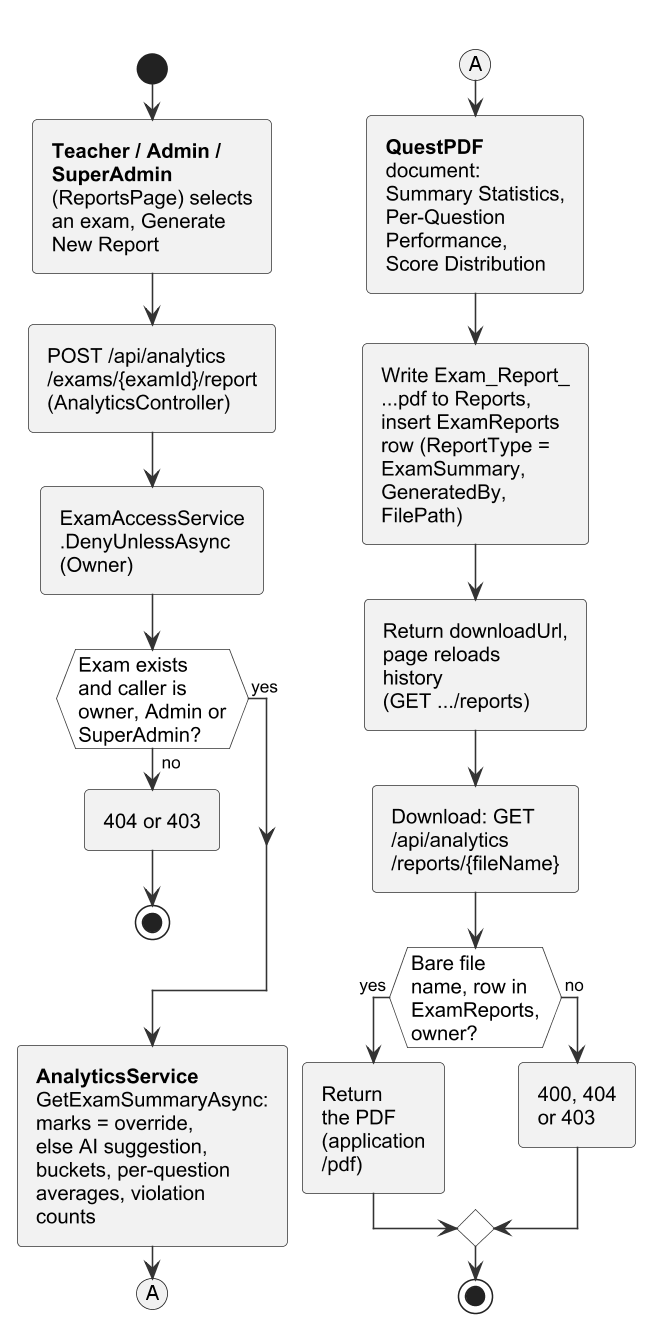
\includegraphics[width=\linewidth]{Figures/activity_report.png}
\caption{Activity Diagram of PDF Report Generation}
\label{fig:activity_report}
\end{minipage}\hfill
\begin{minipage}[t]{0.48\linewidth}
\centering
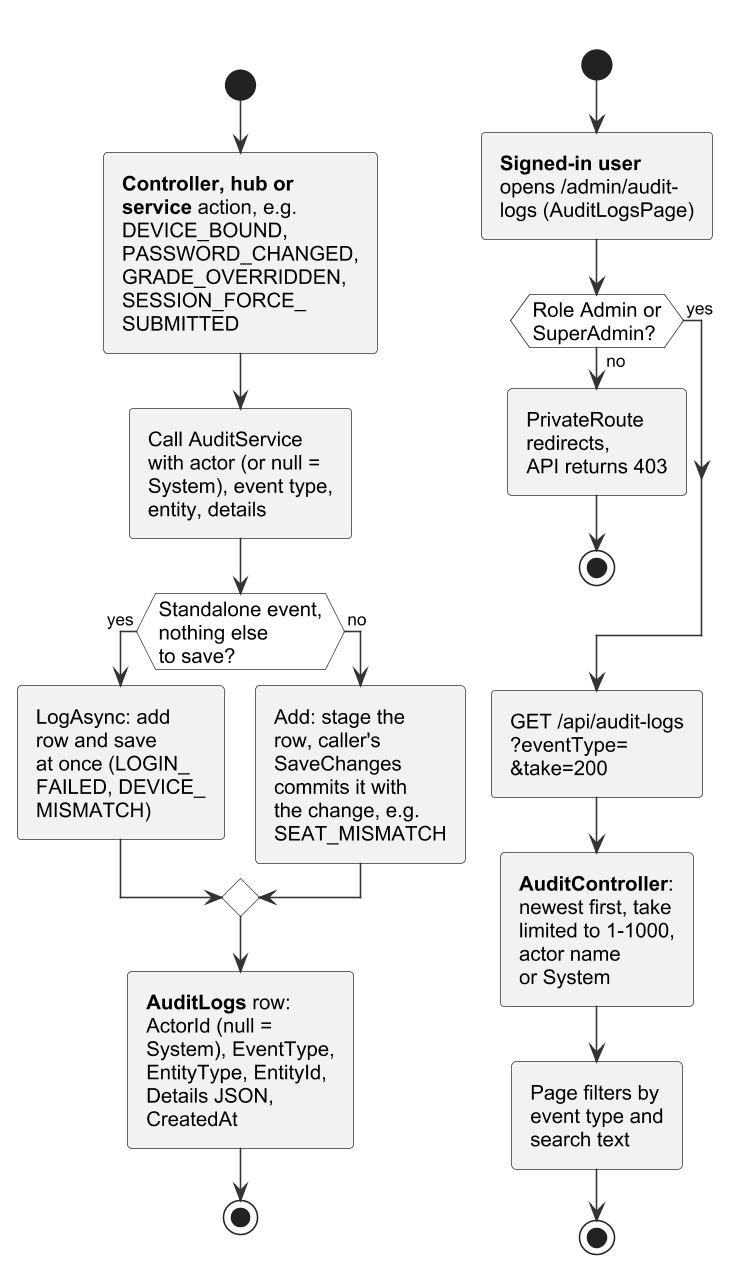
\includegraphics[width=\linewidth]{Figures/activity_audit.png}
\caption{Activity Diagram of Audit Logging}
\label{fig:activity_audit}
\end{minipage}
\end{figure}

\subsection{Communication Diagram}
\begin{sloppypar}
A communication diagram shows the objects in one interaction and their numbered messages \cite{communication_diagram_boardmix}. Figure~\ref{fig:communication_diagram} follows a violation: the client posts it over REST, \texttt{MonitoringController} stores it and pushes it through the hub to the live monitor, and a teacher or invigilator answers through the hub with a warning or force-submit. The hub checks the caller with \texttt{ExamAccessService} and audits the action; a force-submit calls \texttt{SubmissionService.FinalizeAsync}. The client picks up the warning or the new session status from its next heartbeat reply, and the warning repeats until it is marked read.
\end{sloppypar}

\begin{figure}[!htbp]
\centering
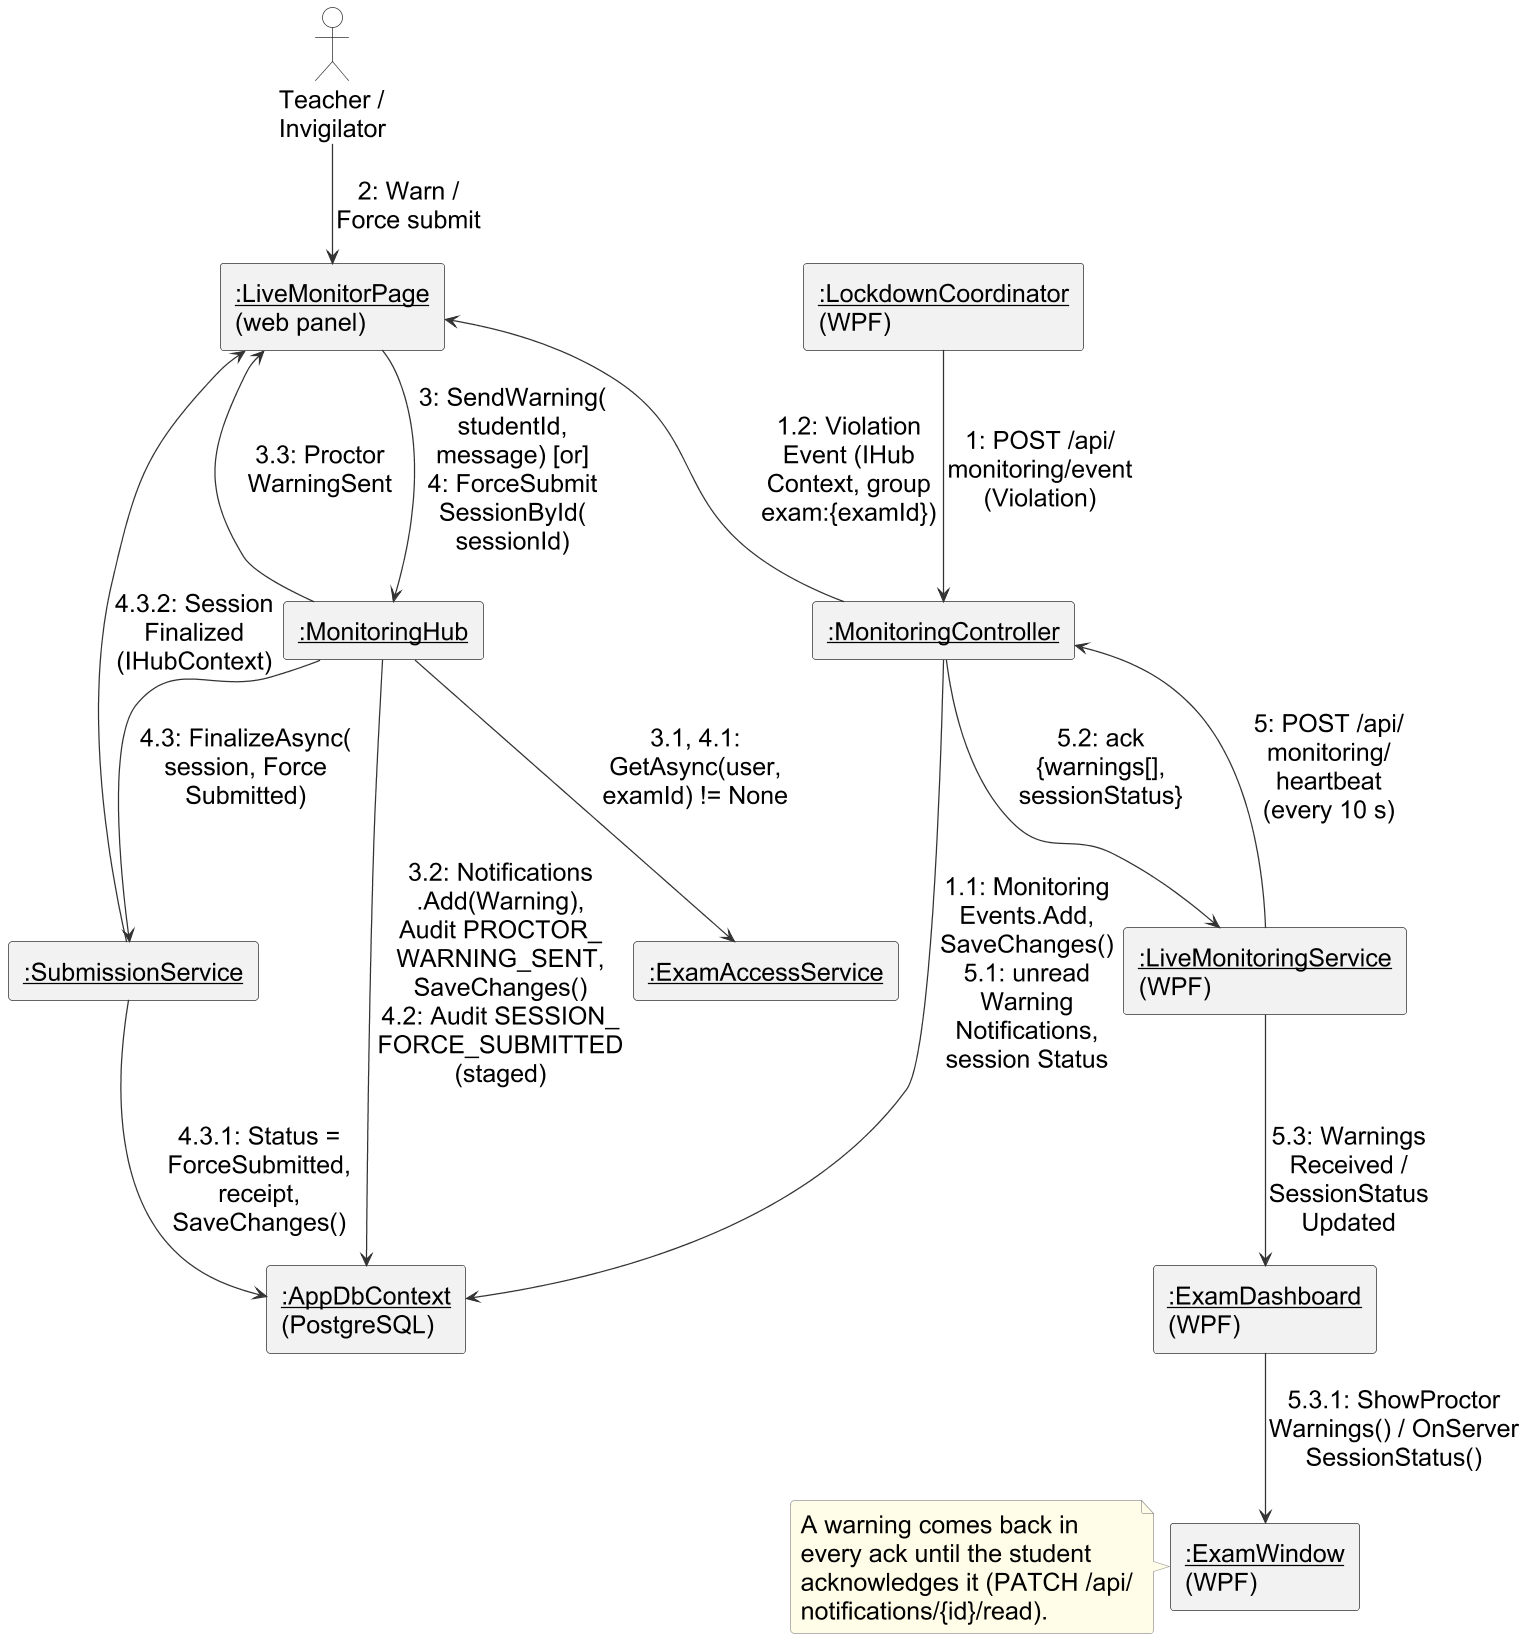
\includegraphics[width=0.97\linewidth]{Figures/communication_diagram.png}
\caption{Communication Diagram of Violation Alerts and Staff Response}
\label{fig:communication_diagram}
\end{figure}

\subsection{Sequence Diagrams}
A sequence diagram shows the messages between participants in time order \cite{sequence_diagram_medium}.

\subsubsection{Login, Logout and Password Change}
\begin{sloppypar}
In Figure~\ref{fig:seq_login} \texttt{AuthController} checks the salted PBKDF2 password hash, the Student role and the device binding (first bind, upgrade of a v1 binding, or \texttt{DEVICE\_MISMATCH}), then returns a JWT and a refresh token. Refresh tokens rotate on every use; reusing an old one revokes its whole family.
\end{sloppypar}

\begin{figure}[!htbp]
\centering
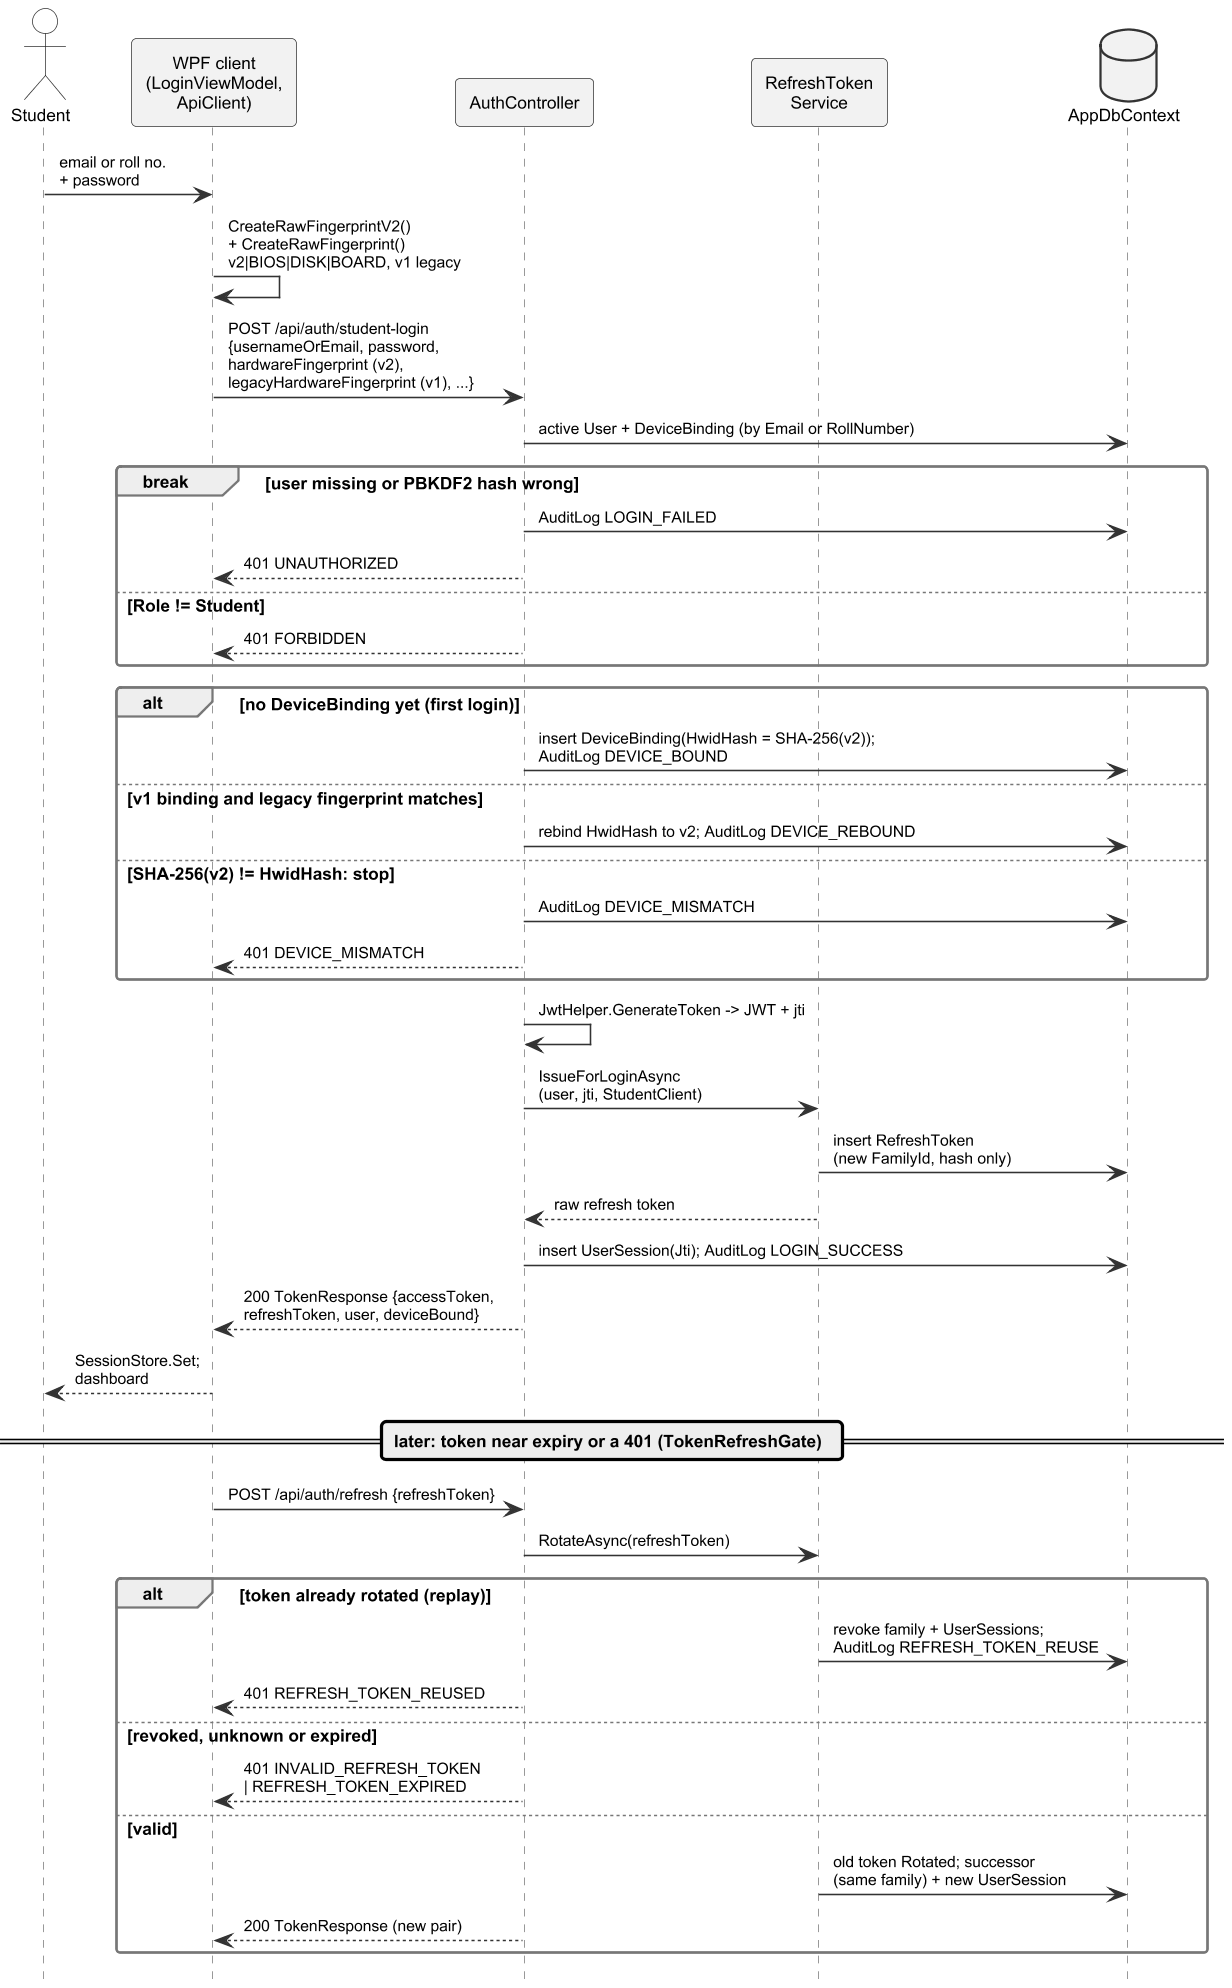
\includegraphics[width=0.9\linewidth]{Figures/seq_login.png}
\caption{Sequence Diagram of Student Login and HWID Verification}
\label{fig:seq_login}
\end{figure}

Logout (Figure~\ref{fig:seq_logout}) revokes the refresh-token family and the session on the server and audits \texttt{LOGOUT}. A staff password change from the web panel (Figure~\ref{fig:seq_change_password}) goes to \url{/api/auth/change-password}, which verifies the current password and a minimum length of 8, ends the user's other sessions, and stores a new salt and PBKDF2 hash; the caller's own session stays valid.

\begin{figure}[!htbp]
\centering
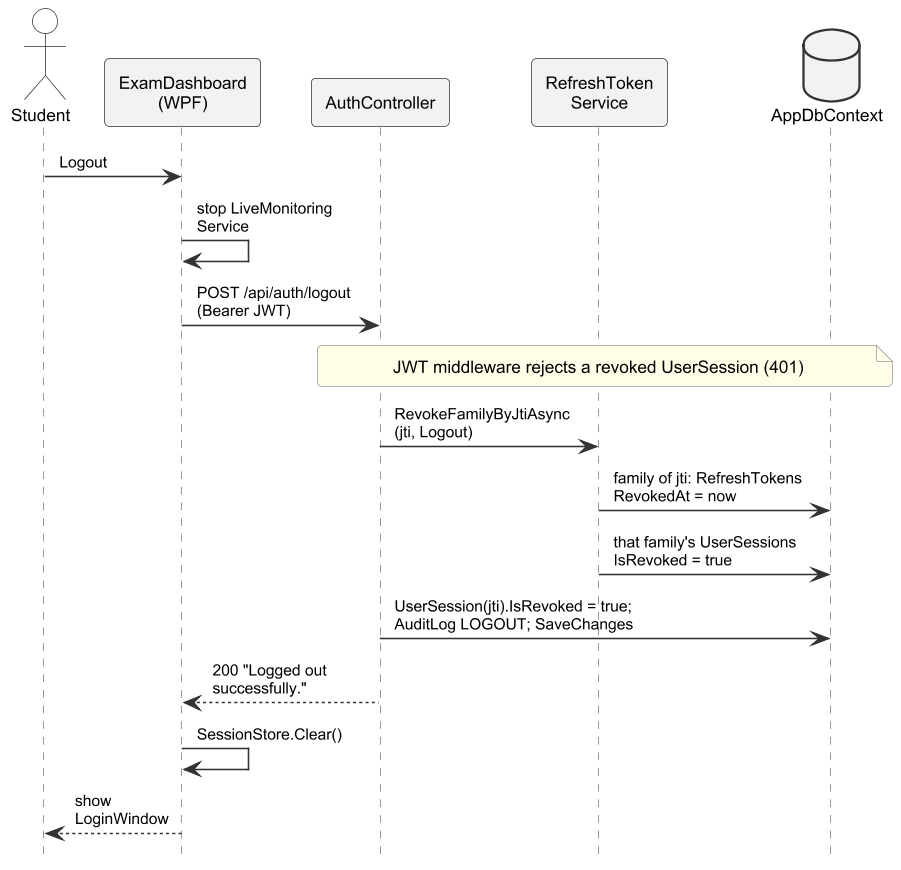
\includegraphics[width=0.65\linewidth]{Figures/seq_logout.png}
\caption{Sequence Diagram of Logout}
\label{fig:seq_logout}
\end{figure}

\begin{figure}[!htbp]
\centering
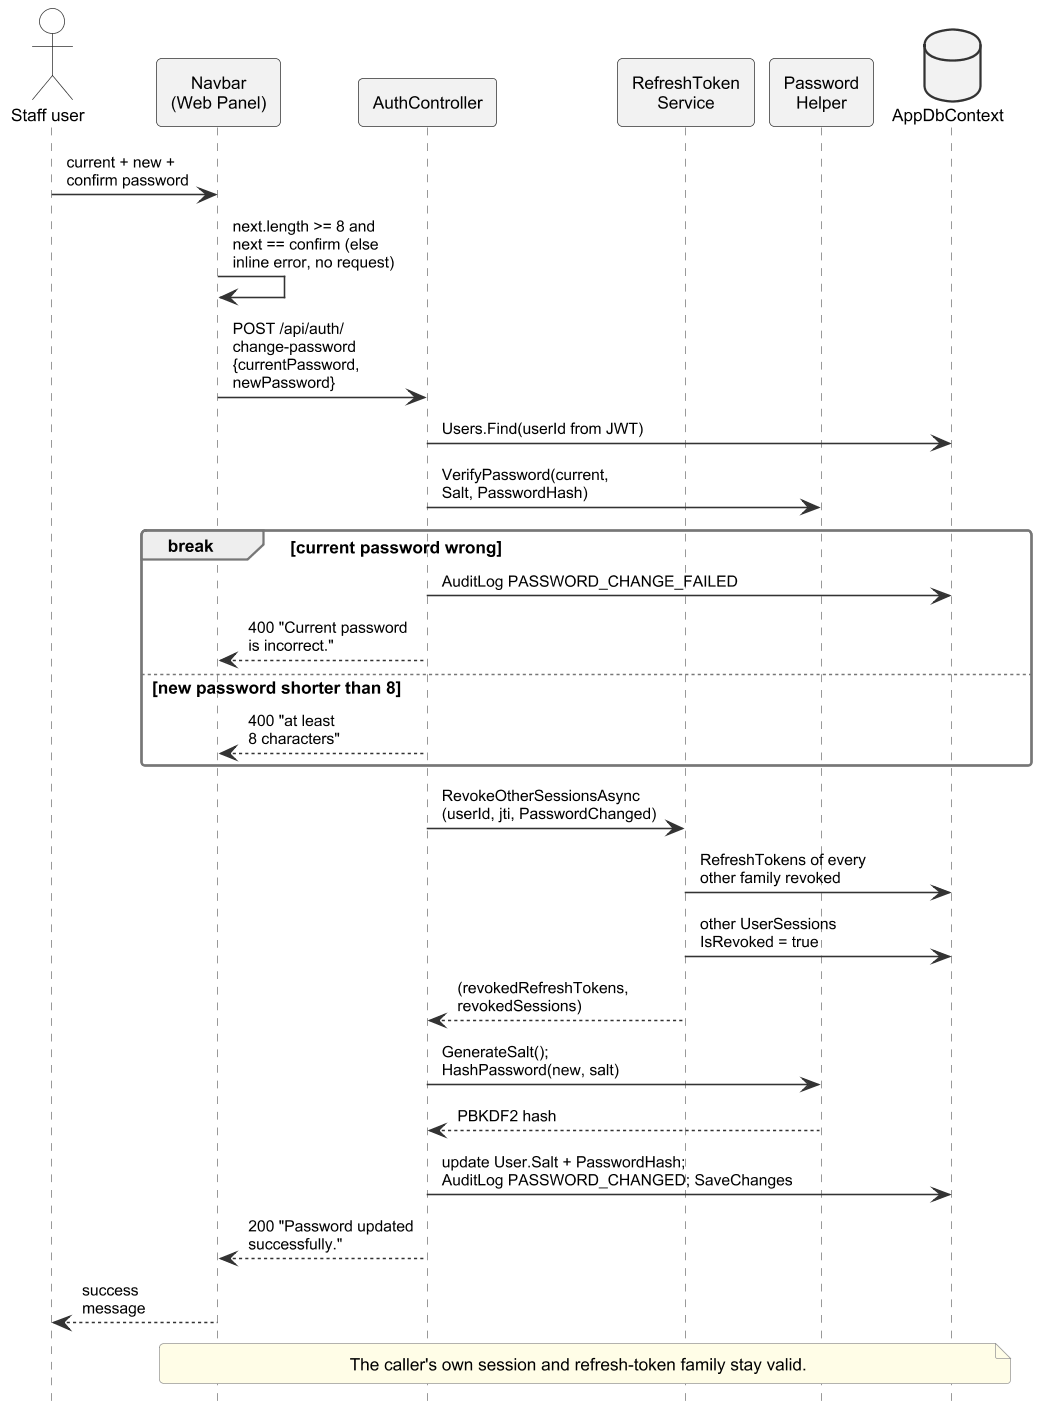
\includegraphics[width=0.9\linewidth]{Figures/seq_change_password.png}
\caption{Sequence Diagram of Password Change}
\label{fig:seq_change_password}
\end{figure}

\subsubsection{Session Timeline and Live Telemetry}
\begin{sloppypar}
To view a student's record (Figure~\ref{fig:seq_view_database}), staff call \texttt{MonitoringEvidenceController}, which checks access through \texttt{ExamAccessService} (owner teacher, assigned invigilator or admin) and returns the session's events (without heartbeats), screenshots, warnings, incidents and audit entries, newest first; each image is then fetched through \texttt{EvidenceStorage}.
\end{sloppypar}

\begin{figure}[!htbp]
\centering
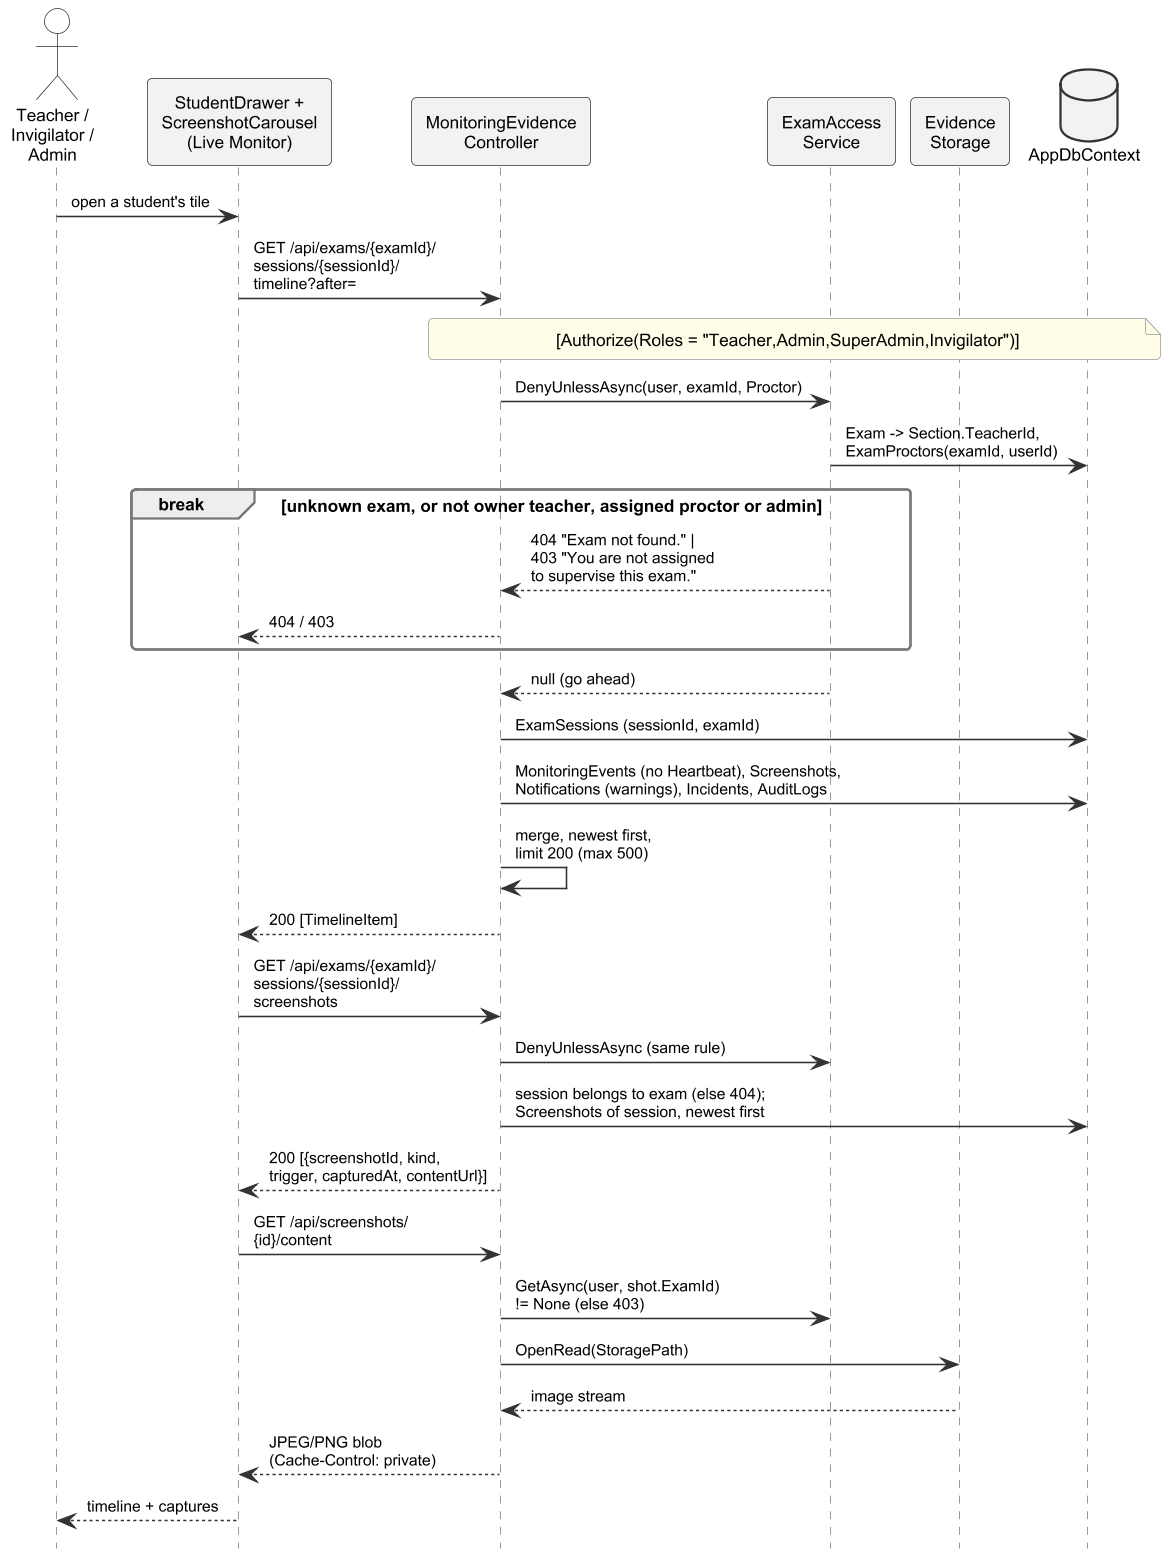
\includegraphics[width=0.9\linewidth]{Figures/seq_view_database.png}
\caption{Sequence Diagram of Viewing a Session Timeline}
\label{fig:seq_view_database}
\end{figure}

In Figure~\ref{fig:seq_telemetry} the start call checks the assignment, seat and readiness gates and creates the session. The client then sends a REST heartbeat every 10 seconds and event batches every 5 seconds. Screen captures are uploaded at random intervals around \texttt{ScreenshotIntervalSeconds} (30--90 seconds by default) and after each violation, plus webcam snapshots when \texttt{RequireWebcam} is set. The server pushes these updates to the hub group, and \texttt{HeartbeatWatchdogService} marks a session disconnected after 30 seconds of silence.

\begin{figure}[!htbp]
\centering
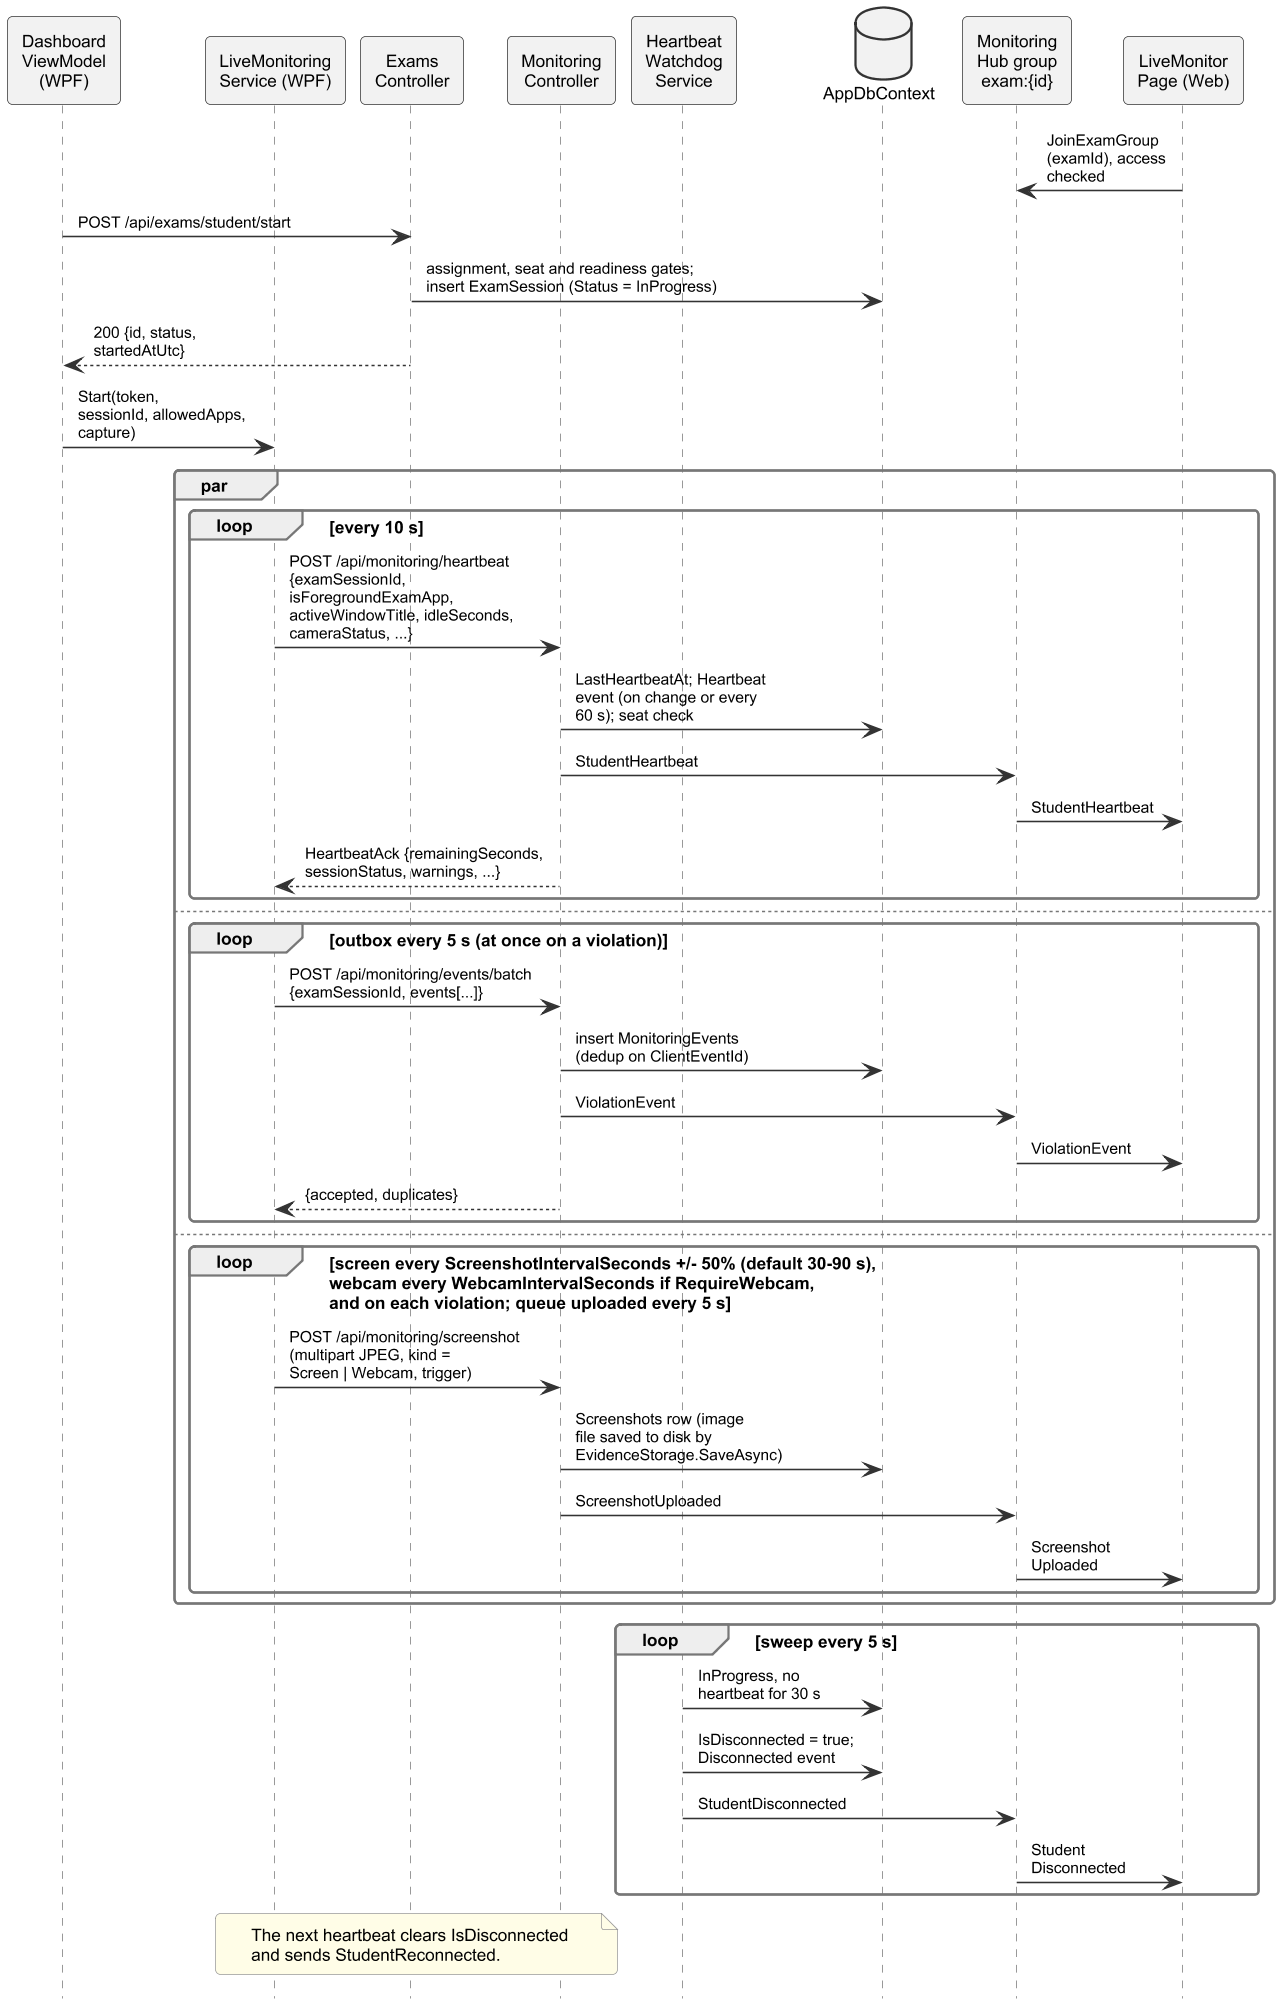
\includegraphics[width=0.9\linewidth]{Figures/seq_telemetry.png}
\caption{Sequence Diagram of Exam Start and Telemetry}
\label{fig:seq_telemetry}
\end{figure}

\subsubsection{Code Execution, Theory Grading and Plagiarism}
\begin{sloppypar}
On submit (Figure~\ref{fig:seq_compilation}) coding answers are staged and queued, and the receipt is returned without waiting. \texttt{GradingWorker} then picks a runner (Docker, else local MinGW), compiles the code once, runs every test case with its time limit and saves the suggested marks in \texttt{AiGradingResults}. Theory answers go to the TF-IDF grader. Coding and theory answers to the same question are compared pairwise (MCQ answers and mock exams are skipped), and pairs at or above the exam's \texttt{PlagiarismThreshold} are stored in \texttt{PlagiarismResults} (Figure~\ref{fig:seq_ai_plagiarism}).
\end{sloppypar}

\begin{figure}[!htbp]
\centering
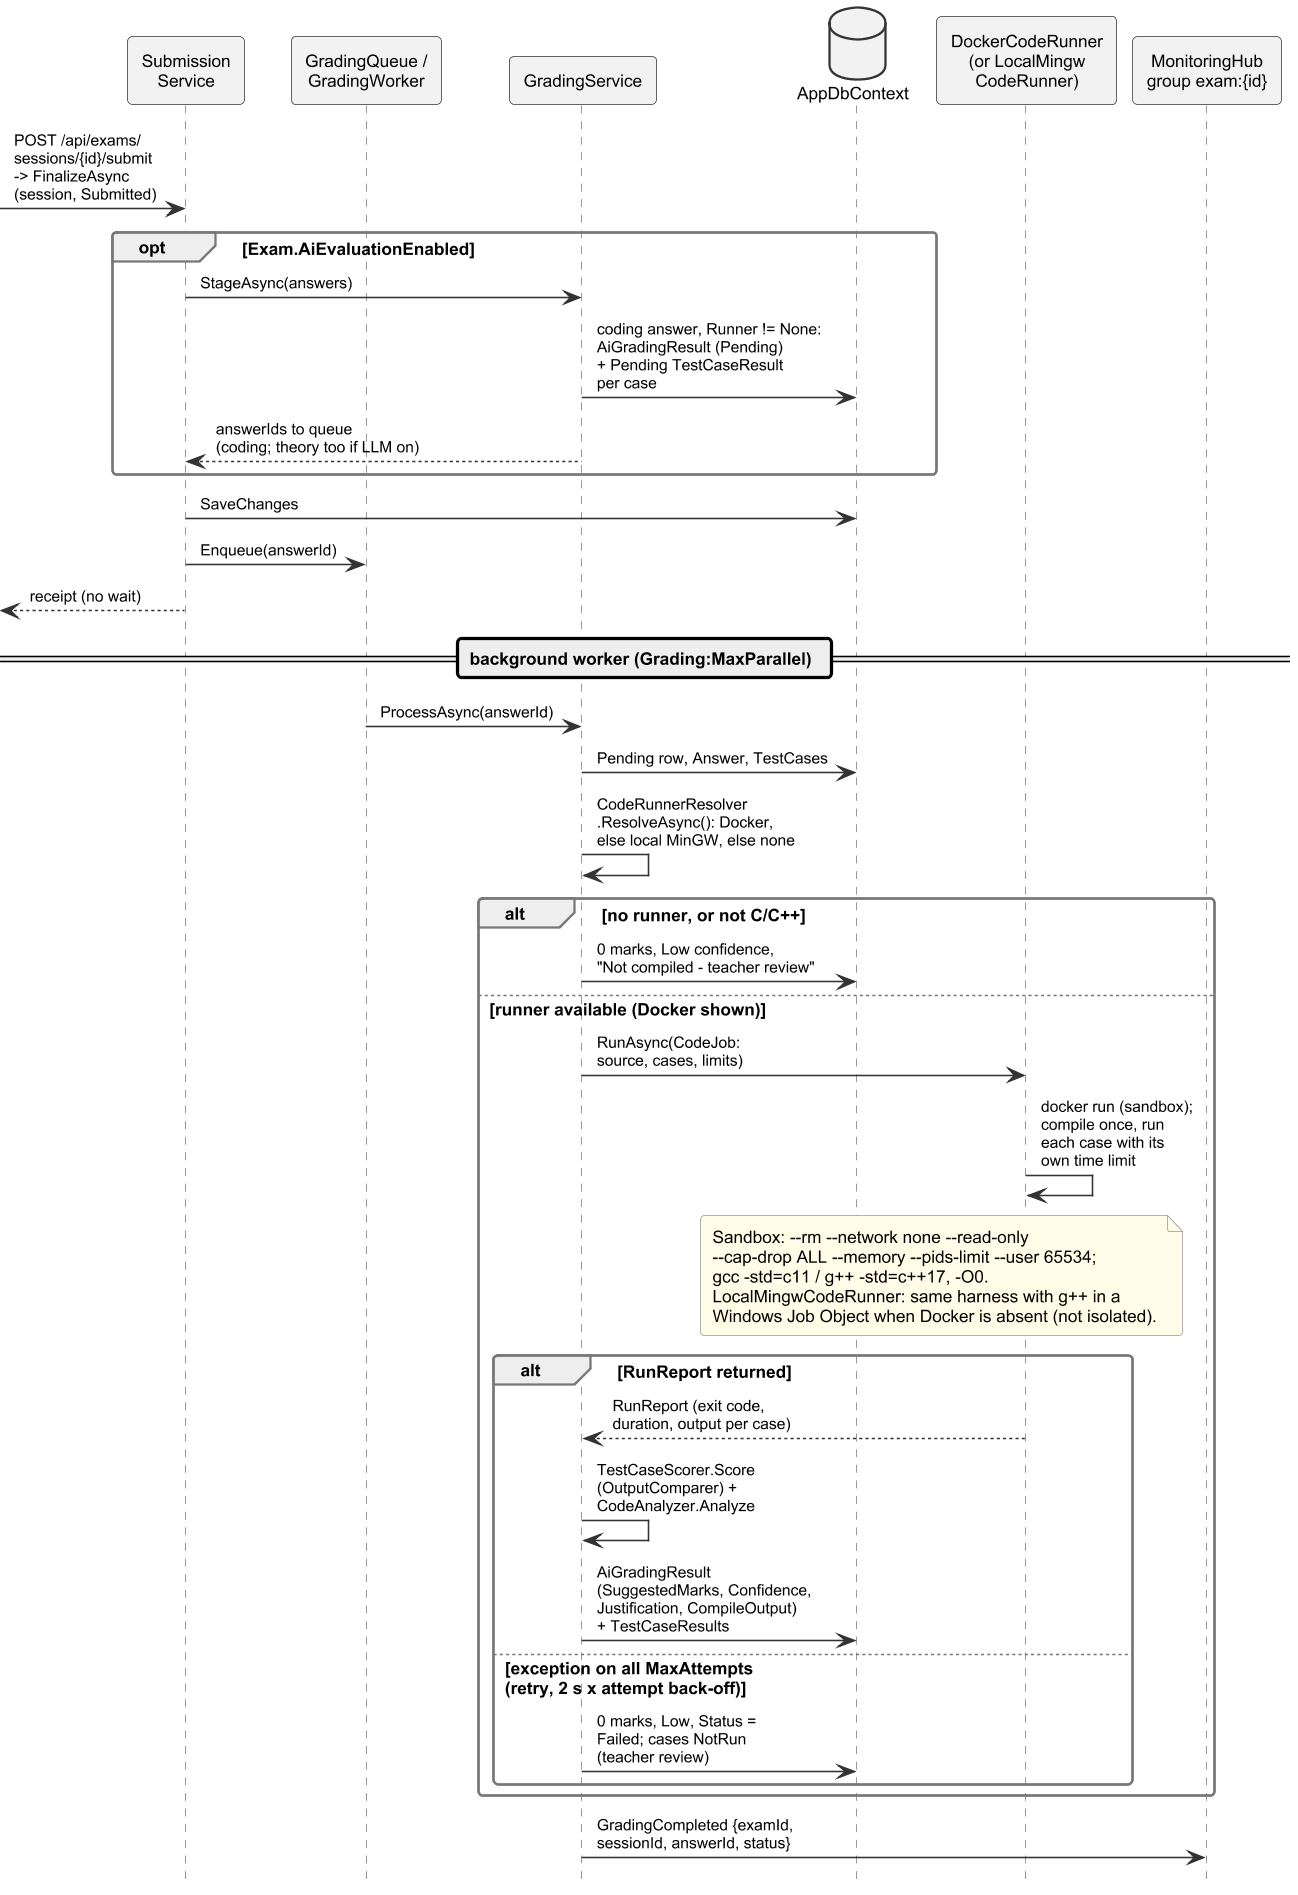
\includegraphics[width=0.97\linewidth]{Figures/seq_compilation.png}
\caption{Sequence Diagram of Sandboxed Code Execution}
\label{fig:seq_compilation}
\end{figure}

\begin{figure}[!htbp]
\centering
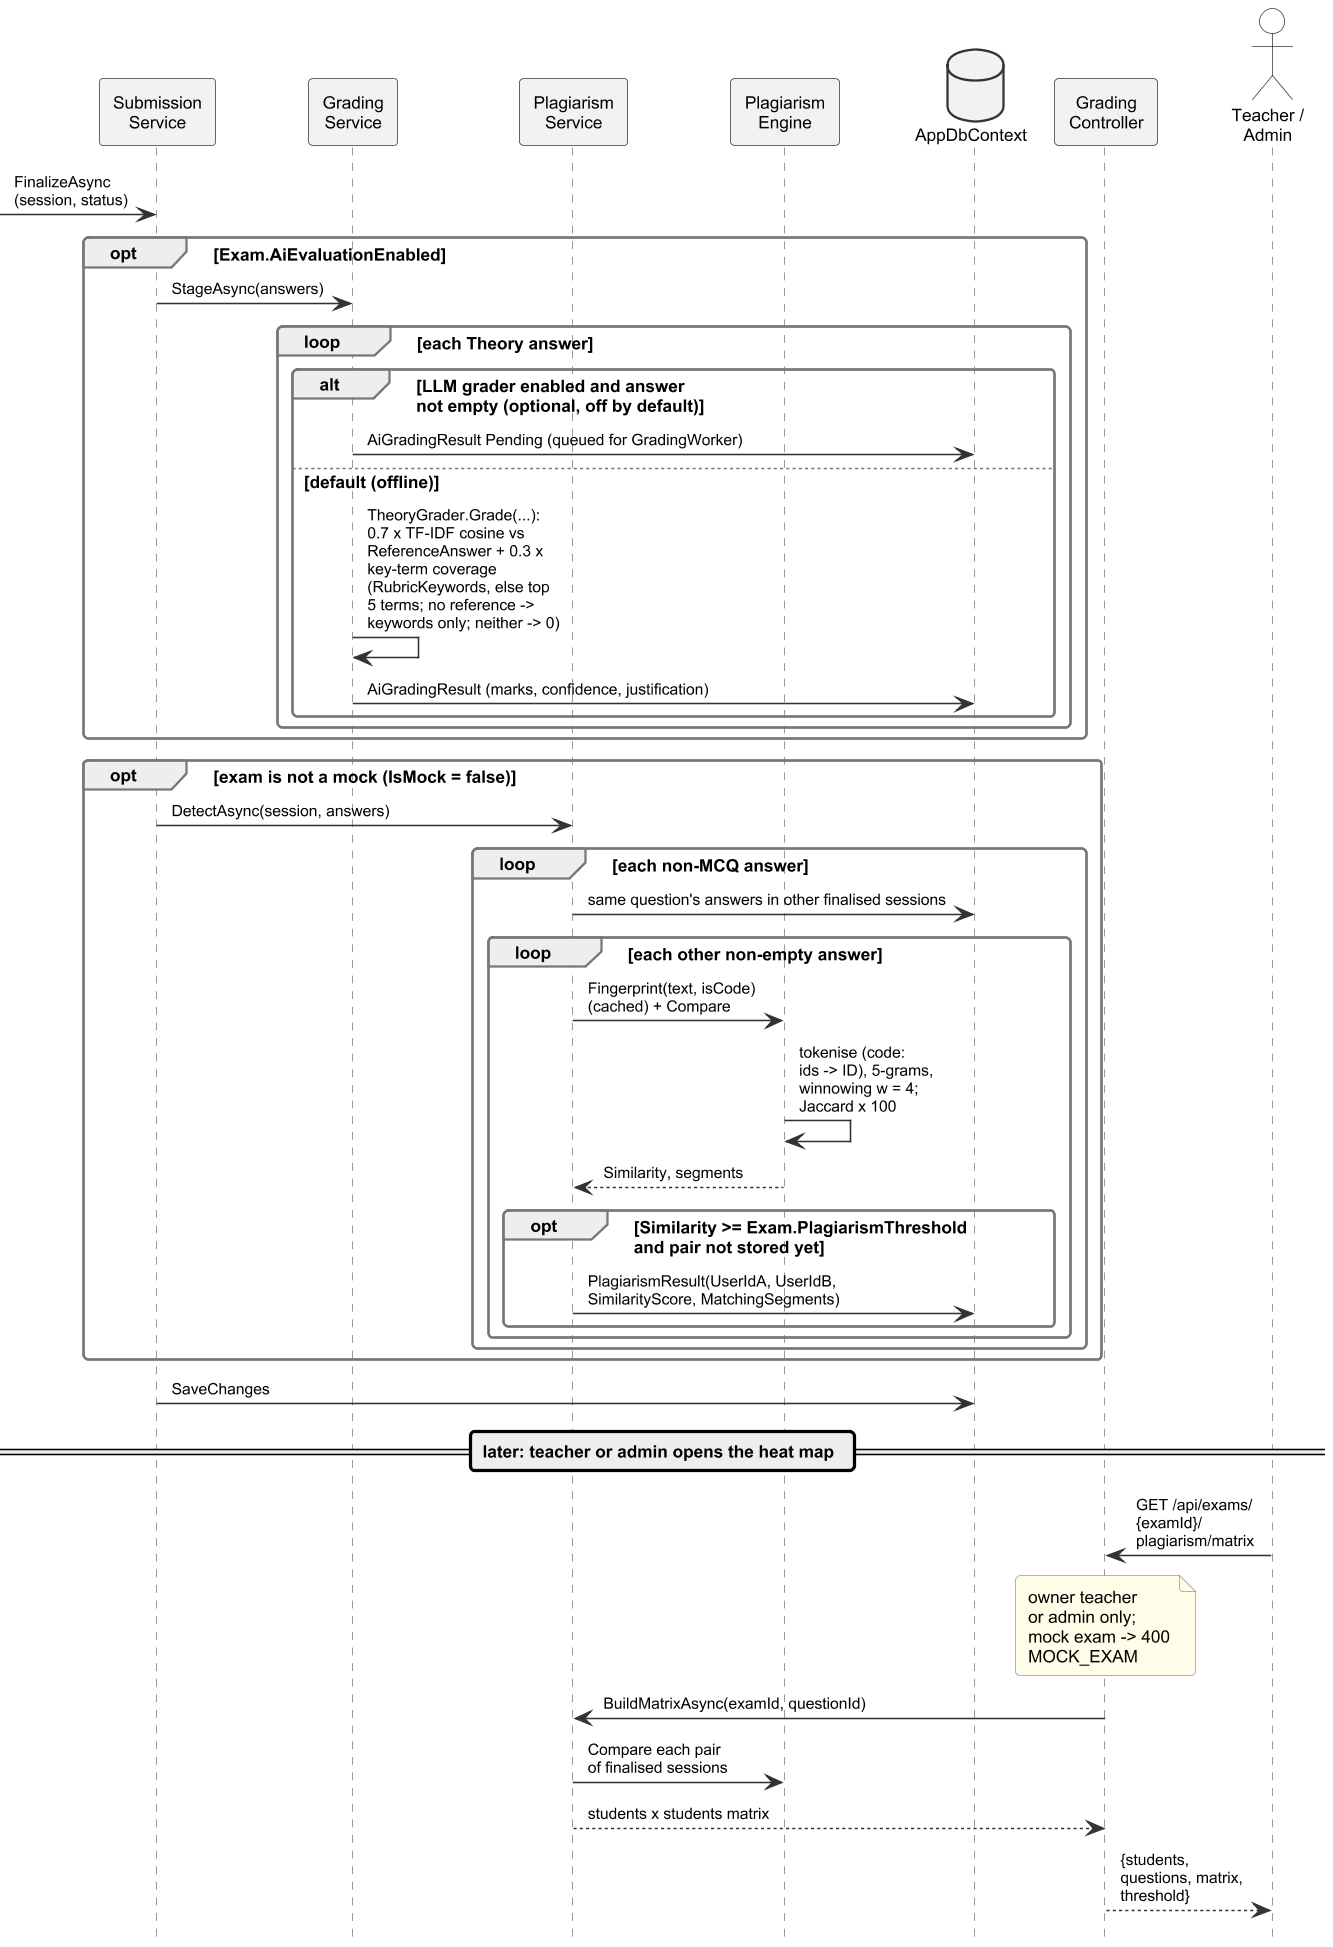
\includegraphics[width=0.97\linewidth]{Figures/seq_ai_plagiarism.png}
\caption{Sequence Diagram of Theory Grading and Plagiarism Check}
\label{fig:seq_ai_plagiarism}
\end{figure}

\subsubsection{Readiness Checks, Mock Test, Lockdown and Recovery}
In Figure~\ref{fig:seq_diagnostics} the client runs the seven readiness checks and posts the result; the server re-checks it, stores a \texttt{ReadinessCheck} row and returns a pass valid for 30 minutes. A mock test uses the same start, save and submit calls as a real exam, in Report mode without the webcam (Figure~\ref{fig:seq_readiness}).

\begin{figure}[!htbp]
\centering
\begin{minipage}[t]{0.48\linewidth}
\centering
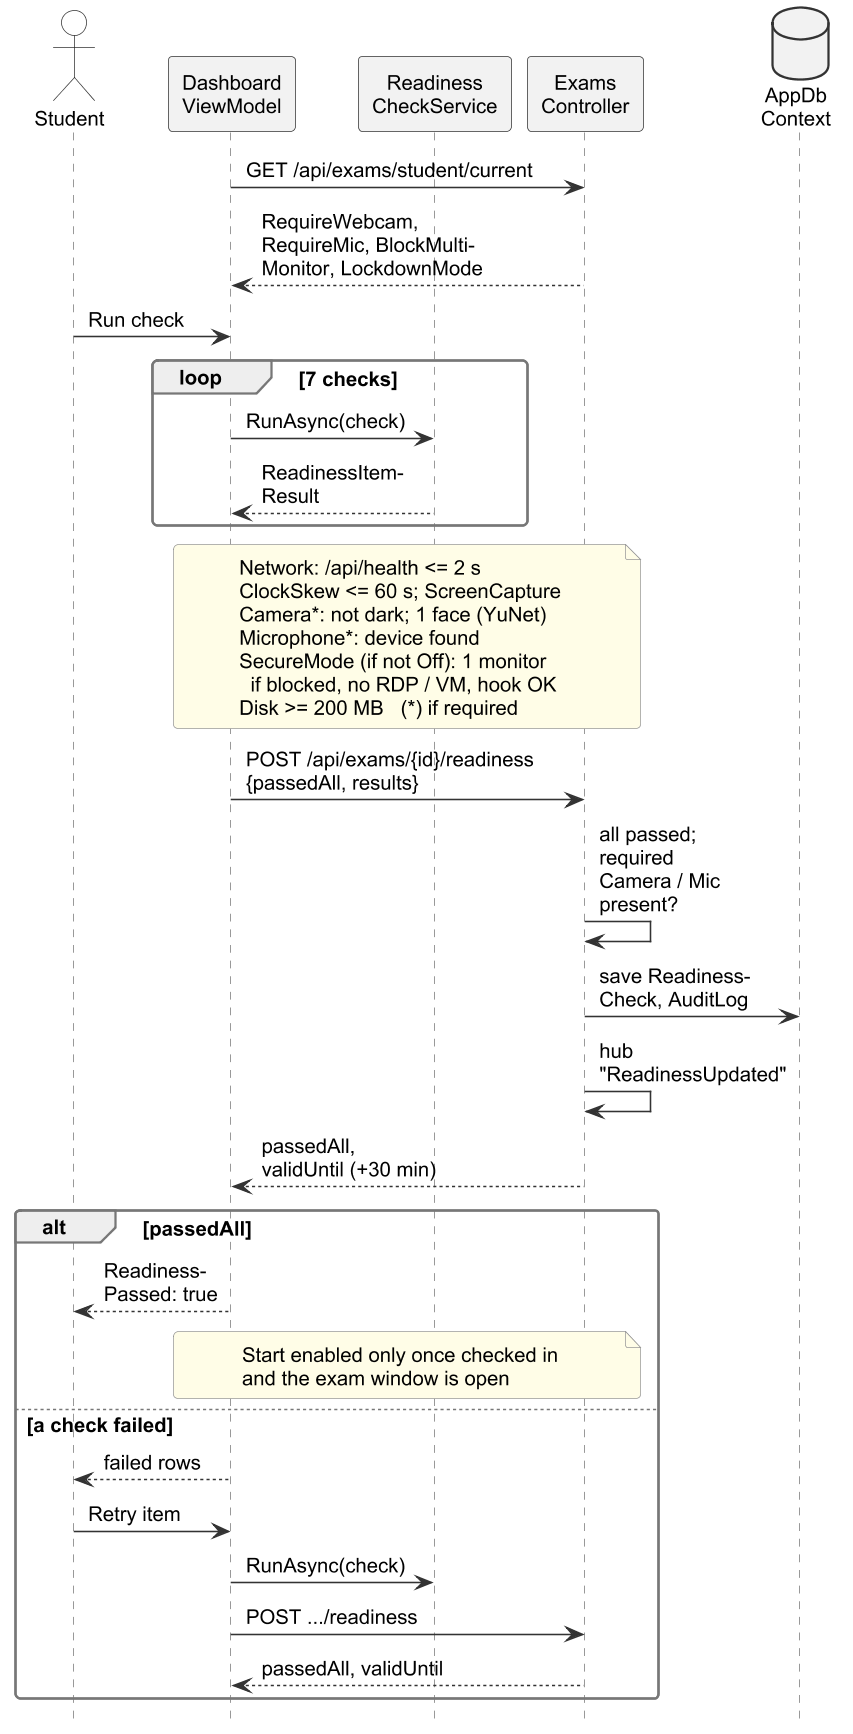
\includegraphics[width=\linewidth]{Figures/seq_diagnostics.png}
\caption{Sequence Diagram of Pre-Exam Readiness Checks}
\label{fig:seq_diagnostics}
\end{minipage}\hfill
\begin{minipage}[t]{0.48\linewidth}
\centering
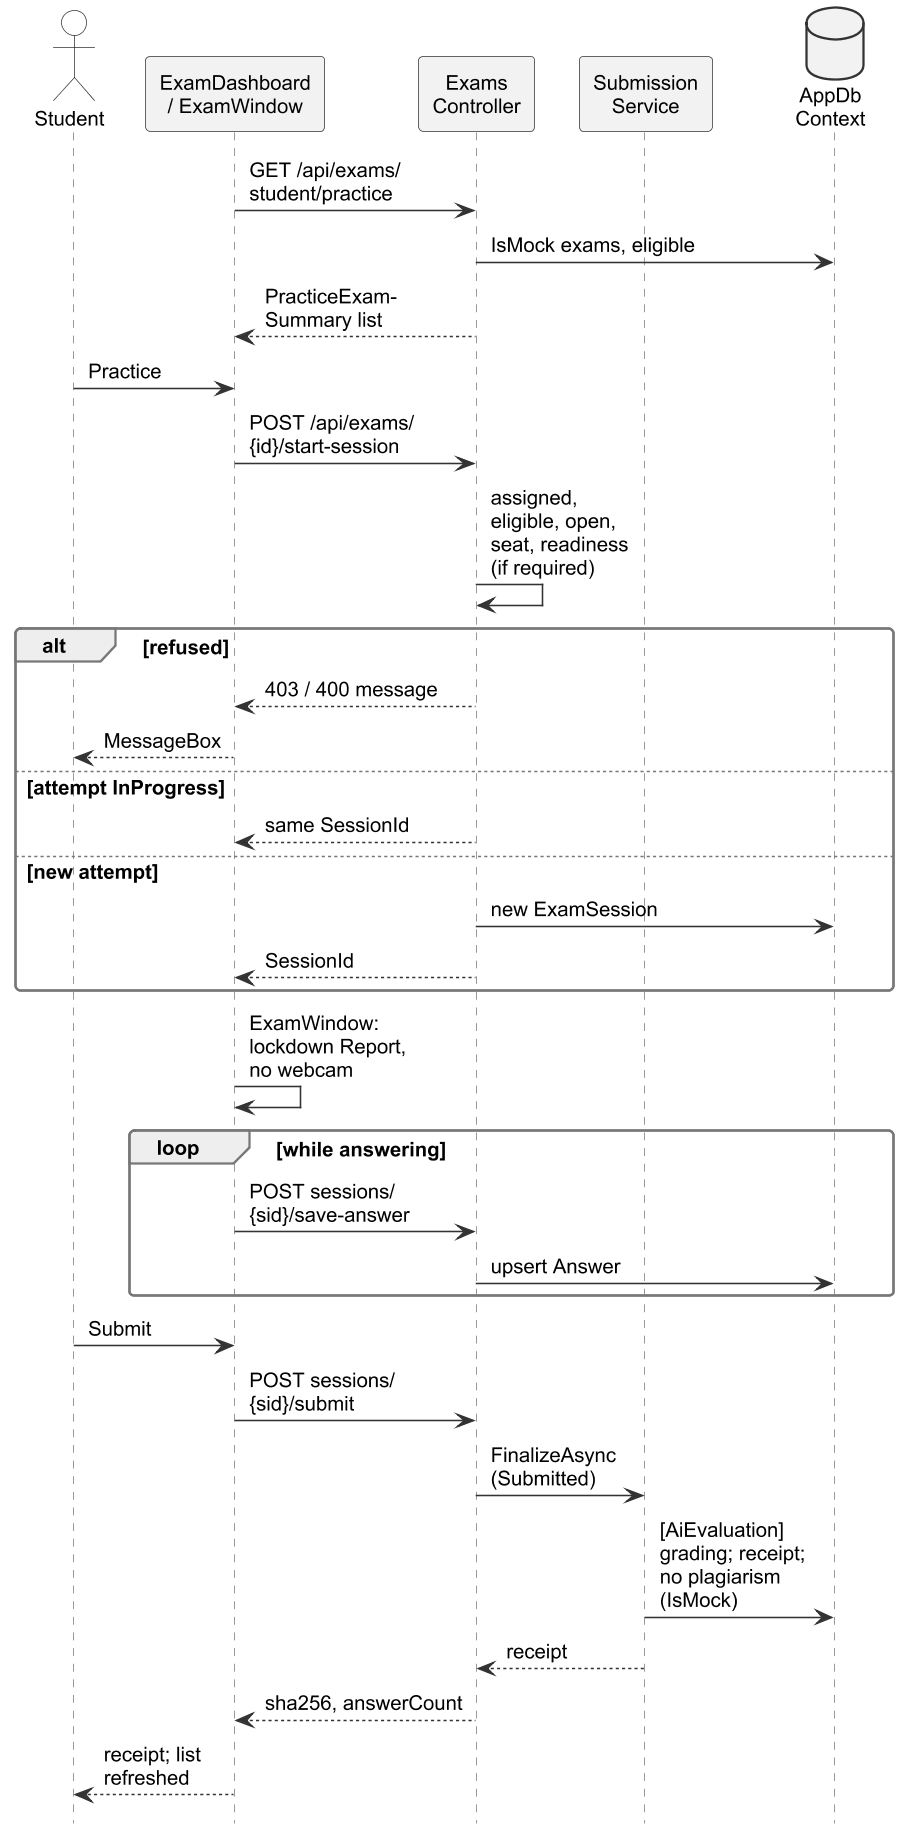
\includegraphics[width=\linewidth]{Figures/seq_readiness.png}
\caption{Sequence Diagram of the Mock Test}
\label{fig:seq_readiness}
\end{minipage}
\end{figure}

At exam start the \texttt{LockdownCoordinator} installs a low-level keyboard hook that blocks Alt+Tab, the Windows keys and similar shortcuts, disables Task Manager through the registry and starts the clipboard, process and device guards. Violations pass a 15-second cooldown and go to the encrypted monitoring outbox (Figure~\ref{fig:seq_lockdown}). Figure~\ref{fig:seq_recovery} shows the save, offline queue, backup and replay calls; after a crash the backup is merged by revision, or ignored if it was tampered with.

\begin{figure}[!htbp]
\centering
\begin{minipage}[t]{0.48\linewidth}
\centering
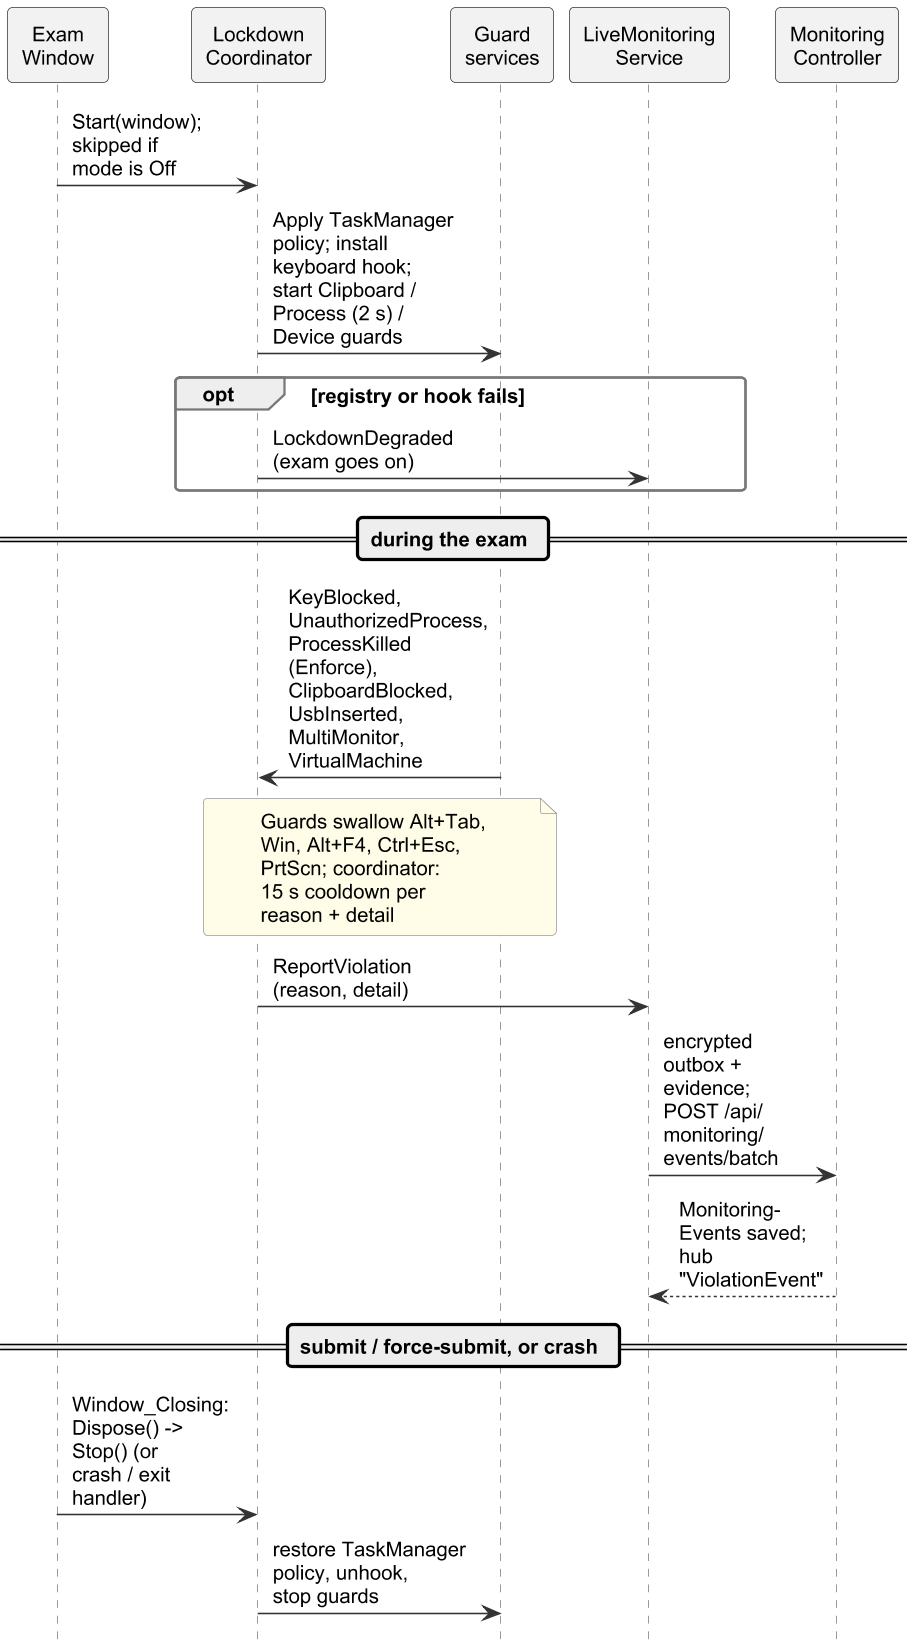
\includegraphics[width=\linewidth]{Figures/seq_lockdown.png}
\caption{Sequence Diagram of Lockdown Enforcement}
\label{fig:seq_lockdown}
\end{minipage}\hfill
\begin{minipage}[t]{0.48\linewidth}
\centering
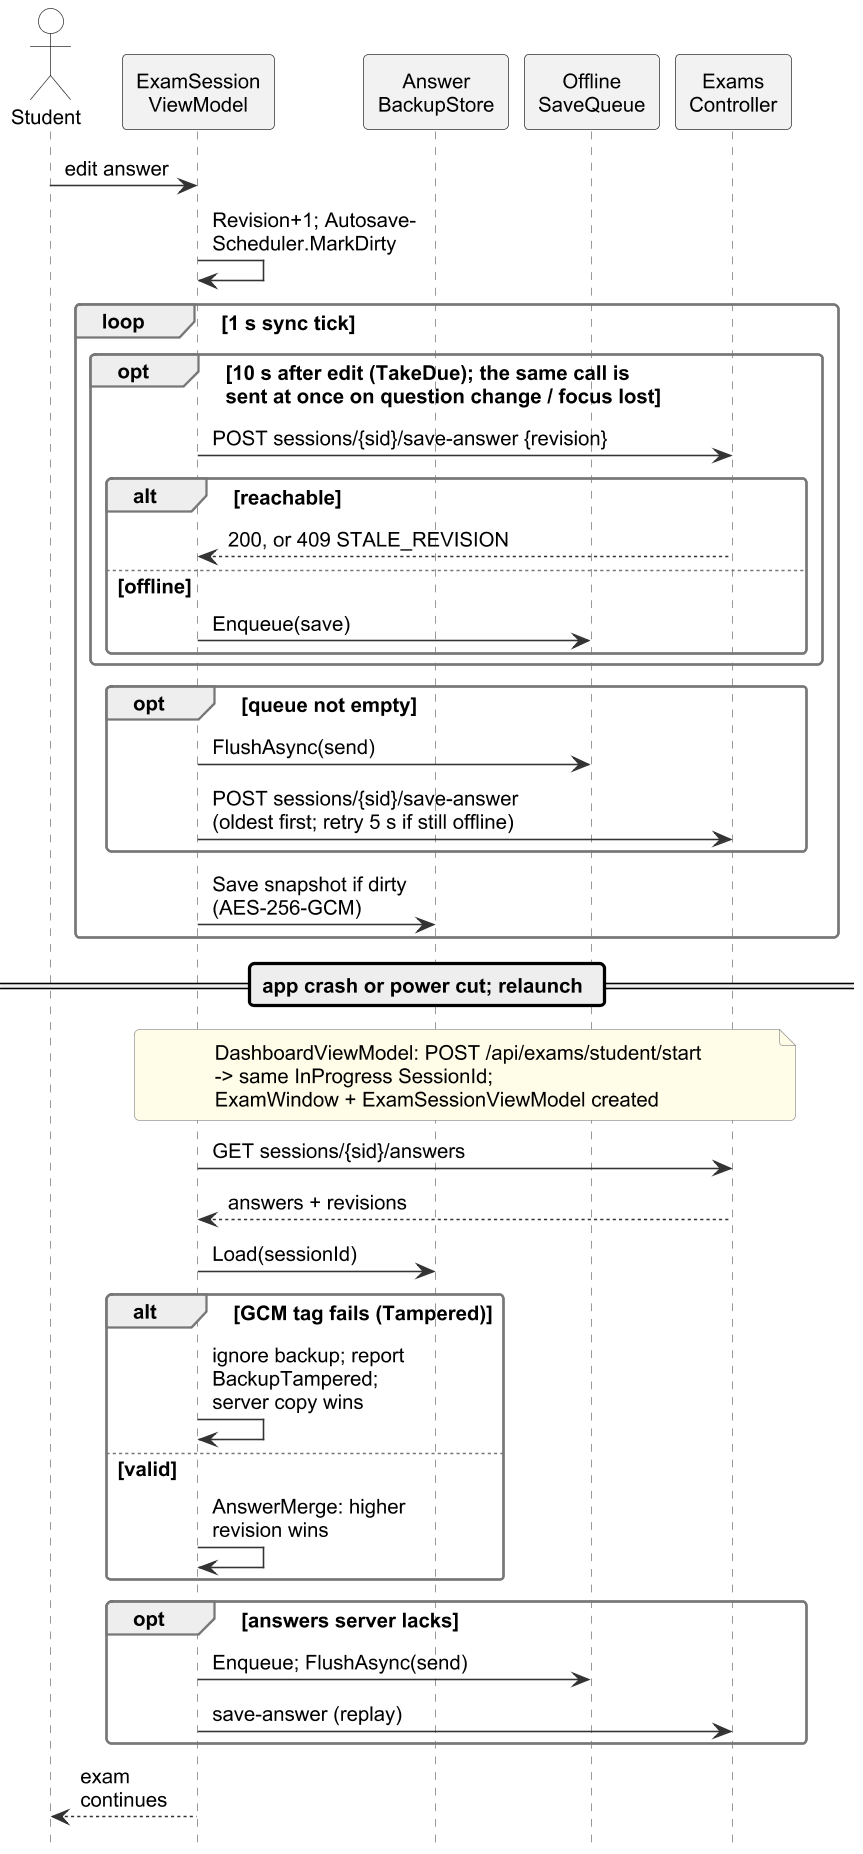
\includegraphics[width=\linewidth]{Figures/seq_recovery.png}
\caption{Sequence Diagram of Auto-Save and Recovery}
\label{fig:seq_recovery}
\end{minipage}
\end{figure}

\subsubsection{Submission, Configuration and Report Export}
On submit (Figure~\ref{fig:seq_submission}) the client first flushes unsent saves. The server checks that the session is the caller's own and in progress, sets it to Submitted with the receipt hash, stages grading and the plagiarism check in one save, then queues the answers; the client verifies the receipt and releases the lockdown. Exam configuration (Figure~\ref{fig:seq_config}) loads the teacher's sections and students, then makes one create or update call to \texttt{ExamsController} carrying the questions and test cases.

\begin{figure}[!htbp]
\centering
\begin{minipage}[t]{0.48\linewidth}
\centering
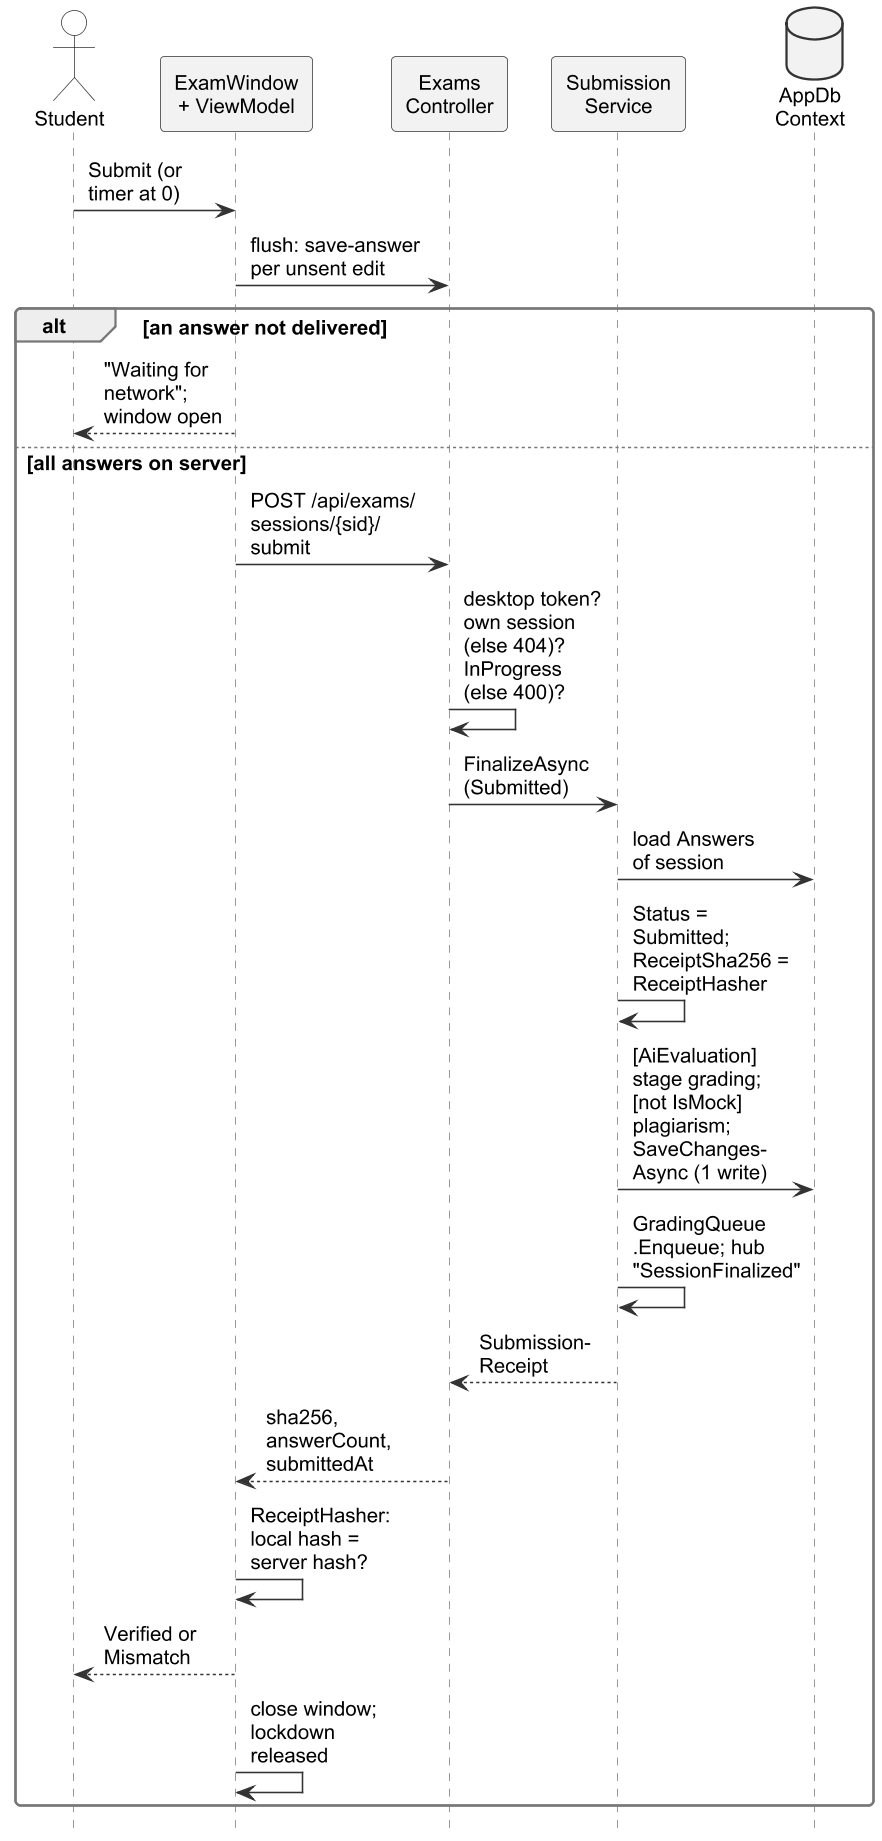
\includegraphics[width=\linewidth]{Figures/seq_submission.png}
\caption{Sequence Diagram of Exam Submission}
\label{fig:seq_submission}
\end{minipage}\hfill
\begin{minipage}[t]{0.48\linewidth}
\centering
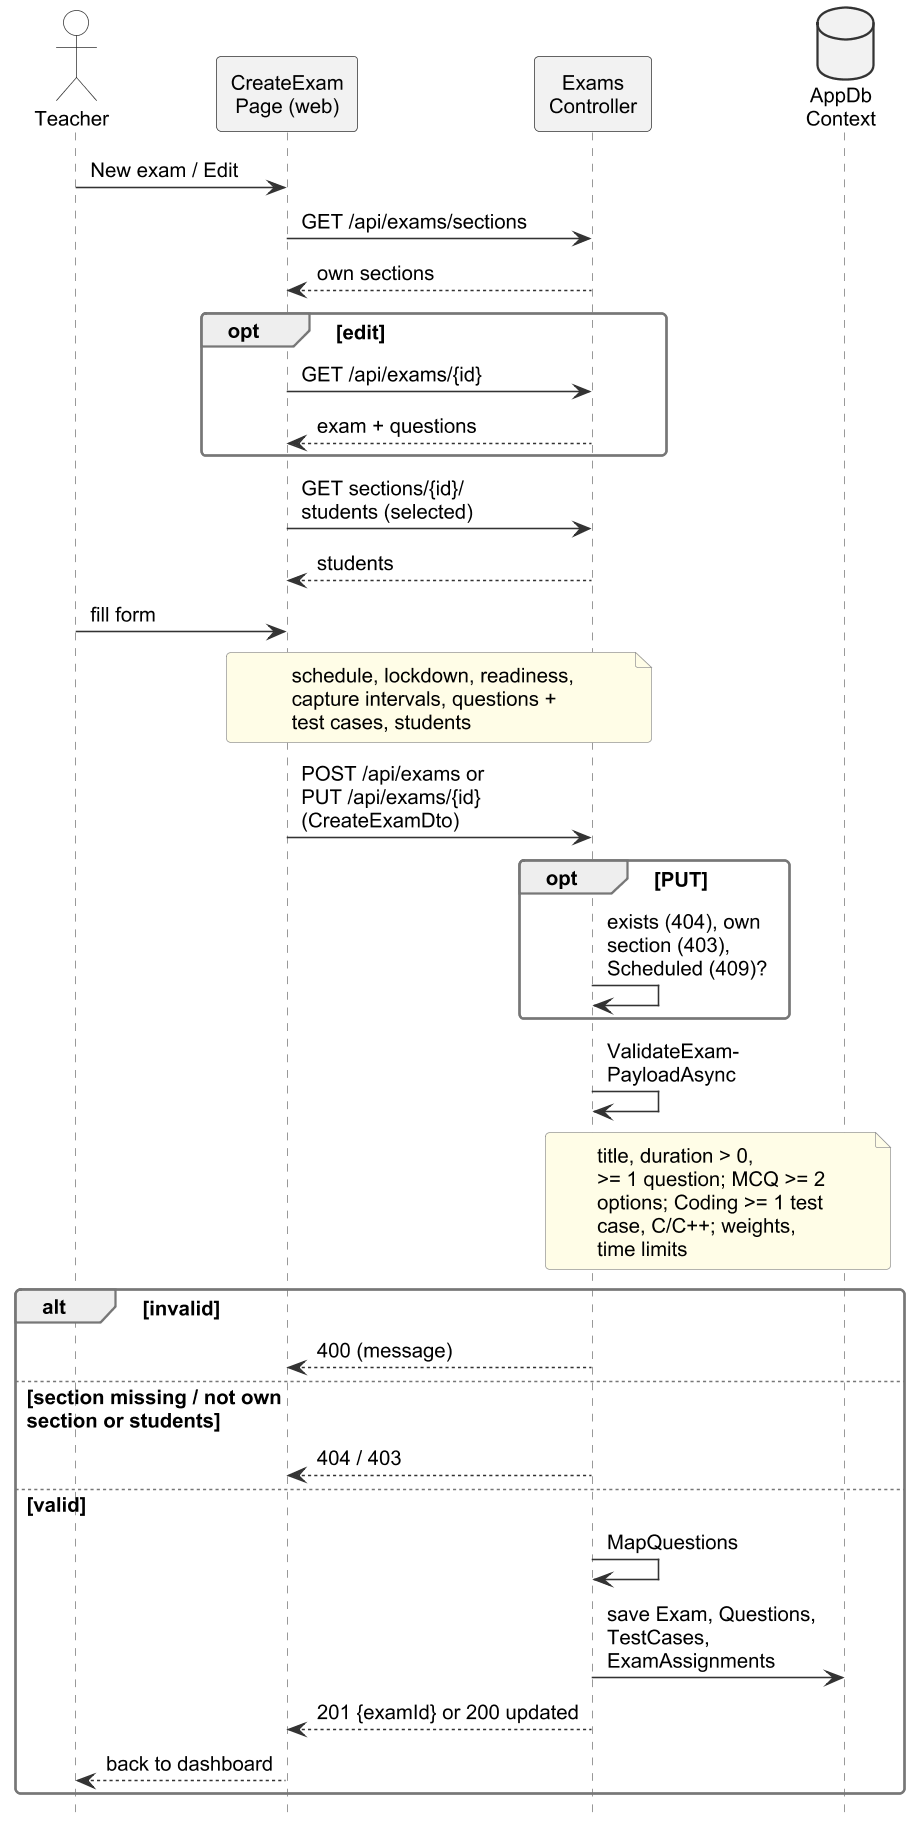
\includegraphics[width=\linewidth]{Figures/seq_config.png}
\caption{Sequence Diagram of Exam Configuration}
\label{fig:seq_config}
\end{minipage}
\end{figure}

For a report (Figure~\ref{fig:seq_audit}) the panel calls \texttt{AnalyticsController}, which checks exam ownership, renders the PDF with QuestPDF, adds an \texttt{ExamReport} row and returns a download link. The download re-checks the file name and ownership; no audit entry is written.

\begin{figure}[!htbp]
\centering
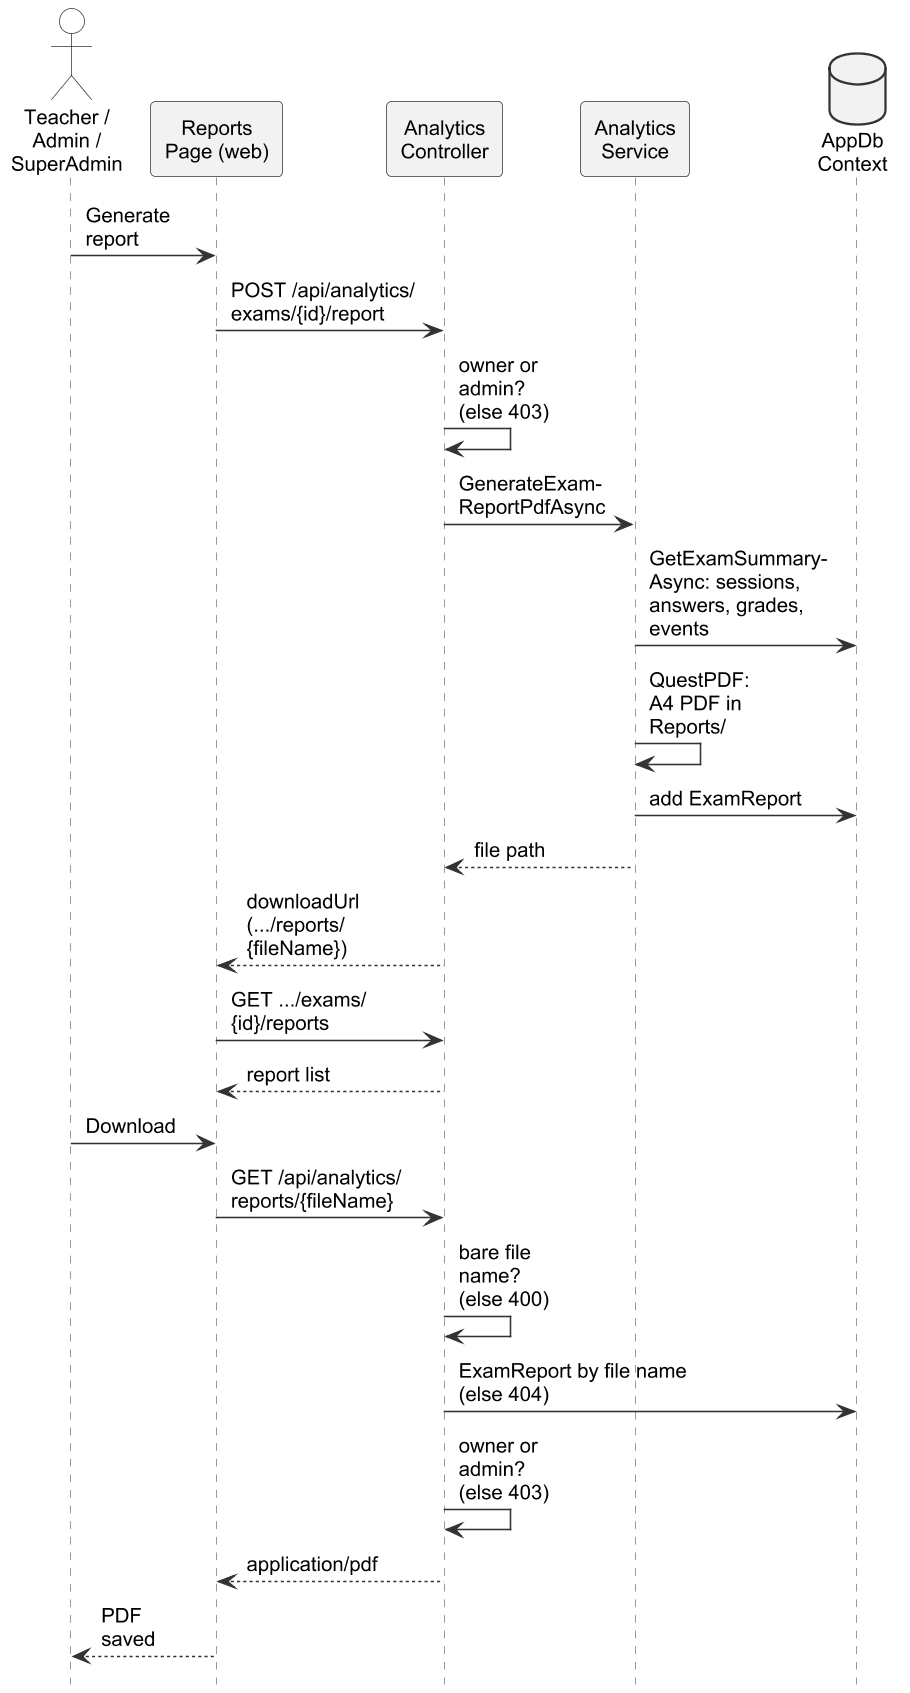
\includegraphics[width=0.6\linewidth]{Figures/seq_audit.png}
\caption{Sequence Diagram of Report Export}
\label{fig:seq_audit}
\end{figure}

\renewcommand{\floatpagefraction}{0.5}
